\chapter{Dataset Construction}
\label{chap:dataset-construction}

As determined in Section~\ref{sec:related-work-routing}, two synthetic datasets are generated to answer the research questions: one for single-turn requests, one for multi-turn requests. A large language model is prompted to generate the requests for a coordinator agent, each routable to exactly one of the available sub-agents. This chapter describes the design of these datasets, the pipeline that generates them, and the analysis used to validate them. Section~\ref{sec:dataset-overview} presents the taxonomy of sub-agents and the structure of a sample. Section~\ref{sec:generation-pipeline} describes the pipeline stages that produce the requests. Section~\ref{sec:dataset-baselines} and Section~\ref{sec:statistical-validation} report the baselines and the statistical analysis used to confirm that the dataset is suitable for the research questions.

\section{Sub-Agent Taxonomy and Sample Design}
\label{sec:dataset-overview}

Both the single-turn and the multi-turn dataset share the same taxonomy and are built around the same rationale. The only difference is that, in the multi-turn dataset, requests are composed of more than one turn.

In each of the two datasets, every request is chosen to describe a technical scenario in software engineering where a developer asks for guidance on a software system under construction or maintenance. Each request therefore belongs to the same domain and uses similar vocabulary, which responds to the requirement, stated in Section~\ref{subsec:lexical-separability}, that the dataset must be difficult for text-only classifiers. Requests from different domains would make lexical overlap harder to achieve, because the vocabulary would clearly separate the sub-agents: a request about a database migration and a request about a marketing campaign would share little vocabulary regardless of which sub-agent is correct, so their lexical overlap would be minimal and each request would be easily routable.

Software engineering is chosen, among other topics, because the author's familiarity with the domain makes manual review of the requests possible.

\subsection{Constraints}
\label{subsec:constraints-binding-waived}

Each request may express one or more \textbf{constraints}: technical demands that the software system under construction must satisfy, and constraints can conflict with each other. Each constraint is \textbf{owned} by exactly one of the available sub-agents: the constraint states a demand that falls within that sub-agent's concern.

An \textbf{authority figure}, a role named in the request such as a manager, a customer, or a regulator, determines the status of each constraint:

\begin{itemize}
    \item A constraint is \textbf{binding} when an authority figure imposes it. A binding constraint determines the correct sub-agent.
    \item A constraint is \textbf{waived} when an authority figure defers it, for example by moving it to a later milestone. A waived constraint remains part of the request, but it does not determine the correct sub-agent.
\end{itemize}

Exactly one constraint in a request is binding, and every other constraint it expresses is waived. The correct sub-agent is the sub-agent that owns the binding constraint. The sub-agent that owns a waived constraint is called the \textbf{decoy}. Section~\ref{subsec:constraints-example} gives an example of a request that expresses a binding and a waived constraint.

\subsection{Taxonomy}
\label{subsec:sub-agent-taxonomy}

Five sub-agents are used across the single-turn and the multi-turn dataset, within the range required in Section~\ref{subsec:routing-setup}. Table~\ref{tab:sub-agent-taxonomy} lists the five sub-agents and the concern each one owns. A request's correct sub-agent is the one pointed to by its binding constraint. Each sub-agent's name is followed by the identifier used to refer to it for the rest of this chapter.

\begin{table}[H]
    \centering
    \renewcommand{\tabularxcolumn}[1]{m{#1}}
    \begin{tabularx}{\textwidth}{@{}>{\raggedright\arraybackslash}m{6.2cm}>{\raggedright\hyphenpenalty=10000\exhyphenpenalty=10000\arraybackslash}X@{}}
        \toprule
        \textbf{Sub-agent} & \textbf{Binding constraint covered} \\
        \midrule
        \textbf{Scalable Architecture} \newline \texttt{scale\_arch} & Designing for concurrency, or for spreading the work across more machines, beyond the load the system carries today. \\ \addlinespace[0.9em]
        \textbf{Legacy Compatibility} \newline \texttt{legacy\_compat} & An existing API contract, client, or dependency that cannot change. \\ \addlinespace[0.9em]
        \textbf{Strict Regulatory Compliance} \newline \texttt{strict\_compliance} & A security, privacy, or regulatory rule. \\ \addlinespace[0.9em]
        \textbf{Resource Optimization} \newline \texttt{resource\_opt} & A fixed CPU, memory, or cost ceiling. \\ \addlinespace[0.9em]
        \textbf{Time-to-Market} \newline \texttt{time\_to\_market} & A fixed ship date or delivery deadline that cannot move. \\
        \bottomrule
    \end{tabularx}
    \caption[The five sub-agents and the binding constraint each one covers]{The five sub-agents and the binding constraint each one covers.}
    \label{tab:sub-agent-taxonomy}
\end{table}

\clearpage
\subsection{Example}
\label{subsec:constraints-example}

The following example illustrates a request that introduces a conflict between two constraints.

\begin{scenariobox}{Request}
\textit{``The events table and the reporting API share a connection pool today and it falls over under spikes. \binding{Our architect requires them separated into services with independent database access so instances scale out without contending for the same resources.} \waived{The analytics team would rather the API's response format stayed unchanged for existing clients, though they have agreed to a parallel-format window if we need to change it.} Where I would like input is the boundary itself: what belongs in the reporting service versus the events service, and how the read path crosses it.''}
\end{scenariobox}

\begin{table}[H]
    \centering
    \renewcommand{\tabularxcolumn}[1]{m{#1}}
    \begin{tabularx}{\textwidth}{@{}l>{\raggedright\hyphenpenalty=10000\exhyphenpenalty=10000\arraybackslash}X>{\raggedright\hyphenpenalty=10000\exhyphenpenalty=10000\arraybackslash}X@{}}
        \toprule
         & \textcolor{bindingcolor}{\textbf{Binding}} & \textcolor{waivedcolor}{\textbf{Waived}} \\
        \midrule
        \textbf{Constraint} & separate the events table and the reporting API into independently scaling services & keep the API's response format unchanged for existing clients \\ \addlinespace[0.9em]
        \textbf{Authority} & the architect & the analytics team \\ \addlinespace[0.9em]
        \textbf{Reason waived} & --- & agreed to a parallel-format window if the response format needs to change \\ \addlinespace[0.9em]
        \textbf{Owned by} & Scalable Architecture & Legacy Compatibility \\
        \bottomrule
    \end{tabularx}
\end{table}

As the example shows, a request can carry terminology for more than one sub-agent while only one of them is correct. A single binding constraint per request ensures exactly one correct sub-agent, the first requirement from Section~\ref{sec:dataset-requirements}, while the request still carries conflicting terminology.

\clearpage
\subsection{The Collision Graph}
\label{subsec:collision-graph}

Every pair of sub-agents carries a tension: a stated reason why their binding constraints conflict. With five sub-agents, ten pairs are possible, and Table~\ref{tab:collision-graph} lists all of them, from Section~\ref{subsec:sub-agent-taxonomy}, together with the tension each pair carries. The graph is complete: a collision is defined for every pair of sub-agents.

\vspace*{\fill}
\begin{table}[H]
    \centering
    \begin{tabular}{@{}ll>{\raggedright\hyphenpenalty=10000\exhyphenpenalty=10000\arraybackslash}m{9.5cm}@{}}
        \toprule
        \textbf{Sub-agent A} & \textbf{Sub-agent B} & \textbf{Tension} \\
        \midrule
        \texttt{time\_to\_market} & \texttt{scale\_arch} & Meeting the deadline can require hardcoding assumptions that break once the system has to handle far more load. \\ \addlinespace[0.9em]
        \texttt{time\_to\_market} & \texttt{resource\_opt} & Meeting the deadline can require spending more on compute or services than a fixed budget can cover. \\ \addlinespace[0.9em]
        \texttt{time\_to\_market} & \texttt{legacy\_compat} & Meeting the deadline can require changing or bypassing an existing contract that other clients still depend on. \\ \addlinespace[0.9em]
        \texttt{time\_to\_market} & \texttt{strict\_compliance} & Meeting the deadline can require skipping a security or privacy check that a regulation requires. \\ \addlinespace[0.9em]
        \texttt{scale\_arch} & \texttt{resource\_opt} & Scaling the architecture can require running more instances, which raises cost beyond a fixed budget. \\ \addlinespace[0.9em]
        \texttt{scale\_arch} & \texttt{legacy\_compat} & Scaling the architecture can require changing an interface that existing clients depend on. \\ \addlinespace[0.9em]
        \texttt{scale\_arch} & \texttt{strict\_compliance} & Scaling the architecture may require replicating data across more machines, which can move it outside a boundary that strict compliance requires it to stay within. \\ \addlinespace[0.9em]
        \texttt{resource\_opt} & \texttt{legacy\_compat} & Optimizing resources can require removing an abstraction layer, which changes a signature that existing clients depend on. \\ \addlinespace[0.9em]
        \texttt{resource\_opt} & \texttt{strict\_compliance} & Optimizing resources can require cutting a control, such as logging or encryption, that a regulation requires. \\ \addlinespace[0.9em]
        \texttt{legacy\_compat} & \texttt{strict\_compliance} & Preserving old behavior can require keeping a practice, such as an old data-handling method, that a new regulation no longer permits. \\
        \bottomrule
    \end{tabular}
    \caption[Ten colliding constraint pairs among the five sub-agents]{The ten colliding pairs among the five sub-agents, and the tension each pair carries.}
    \label{tab:collision-graph}
\end{table}
\vspace*{\fill}

\clearpage
\subsection{Difficulty Tiers}
\label{subsec:difficulty-tiers}

Samples are generated at three difficulty tiers. The tiers introduce the lexical difficulty required in Section~\ref{subsec:lexical-separability}.

\begin{itemize}
    \item \texttt{plain}: no collision. Only one constraint is stated, and it is binding, so nothing in the request competes with the correct sub-agent. A classifier or a probe is expected to score close to ceiling accuracy on this tier. A low accuracy score would point to a problem in how samples are generated or labeled, rather than to a hard routing decision.
    \item \texttt{natural}: a collision between two sub-agents, as in Table~\ref{tab:collision-graph}. The request talks about both constraints equally, and it says explicitly which one has been waived and by whom. A classifier is expected to score lower on this tier than on the \texttt{plain} tier, because the request also contains the vocabulary of a second sub-agent. An accuracy score equal to or higher than that of the \texttt{plain} tier would point to a waived constraint that is stated too weakly to compete with the binding one.
    \item \texttt{adversarial}: samples are built in pairs. The two requests of a pair share almost all their wording. They differ in only one short clause that names the constraint that has been waived. Each of the two requests names a different constraint as waived, so the pair's two correct sub-agents differ even though the requests are almost identical. A classifier is expected to score lower on this tier than on the \texttt{natural} tier, since most of the words it can use appear in both requests of a pair. An accuracy score equal to or higher than that of the \texttt{natural} tier would point to pairs whose requests differ in more than one clause, so that the remaining wording still identifies the correct sub-agent.
\end{itemize}

Within the \texttt{adversarial} tier, a pair is built around its decoy (Section~\ref{subsec:constraints-binding-waived}): the request presents the decoy's constraint, through its wording and emphasis, as if it were the binding one. The real binding constraint is still stated in the request, but it is written so that it is easy to miss. Four \emph{decoy patterns} are used to write the binding constraint this way, each applying only to the \texttt{adversarial} construction.

These patterns are designed to make routing harder for a coordinator model, not only for the text-only classifiers of Section~\ref{sec:dataset-baselines}.

In each example below, \binding{blue} marks the binding constraint.

\begin{itemize}
    \item \textbf{\texttt{buried\_rule}}: the request asks how to carry out one specific approach, for example a workaround. The binding constraint appears in only one clause of the request, and that clause states why the developer picked that approach instead of a simpler one.

    \begin{scenariobox}{Example -- \texttt{buried\_rule}}
    \textit{``We're trying to split the aggregate computation from the request handler so each can scale independently when we hit 10 million requests a day, though the infrastructure roadmap has that decoupling pushed out to next quarter, but \binding{the legacy API contract locks the response format to a specific JSON field at the top level and we have to keep it working.} Building around that constraint means the aggregation layer stays coupled to the response path. How do we handle the data flow here without rebuilding the response schema from scratch?''}
    \end{scenariobox}

    \item \textbf{\texttt{wrong\_cause}}: the request misleads on the cause of the problem. It confidently claims that the decoy constraint is the problem to be solved, and spends most of its words on it. The binding constraint appears only as a short fact, stated as if it were already obvious, with no explanation given.

    \begin{scenariobox}{Example -- \texttt{wrong\_cause}}
    \textit{``we're hitting memory ceiling hard on the cache, \binding{been blowing past the 512mb heap limit ops set,} and we keep trying to add smarter eviction policies and better compression to squeeze more in there, but the real problem is we can't reshape the response payload the way we need to because every mobile client and partner out there is hardwired to expect the exact json schema we published two years ago, though the api team cleared us to rework the output format if we have to. how do we get the instance footprint back under control without redesigning the whole data contract?''}
    \end{scenariobox}

    \item \textbf{\texttt{late\_mandate}}: the request is about the decoy constraint throughout. The binding constraint arrives at the end, in one flat-toned clause, so it reads as minor.

    \begin{scenariobox}{Example -- \texttt{late\_mandate}}
    \textit{``been looking at our read function design and we're spawning a helper thread for each request that comes in. works fine at current scale but the devops budget owner just locked us into a hard 512mb ceiling and max 64 threads, and they said we can revisit the threading model once we have more headroom in the budget. we have a bunch of production clients calling this function synchronously expecting it to block, and \binding{the platform arch team requires the function signature to stay exactly as-is.} so how do we actually redesign this without breaking the existing interface?''}
    \end{scenariobox}

    \item \textbf{\texttt{bad\_fix}}: the request misleads on the solution. It proposes a concrete fix that serves the decoy constraint, and asks for help carrying it out. The request also states the binding constraint, and that constraint is the reason the proposed fix does not work.

    \begin{scenariobox}{Example -- \texttt{bad\_fix}}
    \textit{``We're building a user profile cache that lives in process memory keyed by user id, and the product manager needs us to ship something working to early adopters in six weeks, with hardcoded cache sizes and TTLs acceptable to hit that deadline, but that timeline got pushed back in the roadmap review. At the same time, \binding{the operations team has set a hard ceiling of 512 megabytes of heap per instance for all caching and won't budge on that limit.} I'm proposing we start with simple fixed-size arrays and stop worrying about memory efficiency for now, which should get us there cheapest. How should we structure this to stay strictly within budget while keeping the implementation straightforward?''}
    \end{scenariobox}
\end{itemize}

\subsection{Personas}
\label{subsec:personas}

Four writing-style categories, called \emph{personas}, are used to generate a request. Personas exist to satisfy the requirement, from Section~\ref{subsec:lexical-separability}, that punctuation and phrasing styles stay balanced across sub-agents: assigning personas independently of the sub-agent prevents a sub-agent from being identifiable by a stylistic marker rather than by its content. Personas are assigned in equal proportions within every difficulty tier.

\begin{itemize}
    \item \textbf{\texttt{normal\_writing}}: the request reads as ordinary professional prose, written in complete sentences with correct punctuation.
    \item \textbf{\texttt{frustrated}}: the request reads as written by someone tired and irritated. Sentences are blunt, some sentences vent about the situation, and some sentences are incomplete, missing a subject or a verb.
    \item \textbf{\texttt{casual}}: the request reads as a relaxed chat message. It uses contractions, starts some sentences with a lowercase letter, and contains occasional small spelling or grammar mistakes.
    \item \textbf{\texttt{extremely\_casual}}: the request reads as a message typed in a hurry. It is mostly lowercase, uses minimal punctuation, and shortens words into abbreviations.
\end{itemize}

\subsection{Multi-turn Derivation}
\label{subsec:multiturn-derivation}

The multi-turn dataset uses a fixed number of turns, following the requirement in Section~\ref{subsec:multiturn-setting}. Every multi-turn sample starts with a developer message, and the developer and the coordinator then alternate messages. The conversation ends on a developer message, left unanswered, and the whole conversation is routed based on it. Together with the developer messages and the coordinator responses before it, this last message forms a fixed number of turns for every multi-turn sample. Conversation length therefore does not become a second difficulty axis alongside the three tiers. Each sample contains two full developer and coordinator turns, followed by the final, unanswered developer message, as Figure~\ref{fig:multiturn-alternation} shows.

\begin{figure}[H]
    \centering
    \begin{tikzpicture}[
        node distance=6mm,
        every node/.style={font=\small},
        box/.style={draw, rounded corners, align=center, minimum height=8mm, minimum width=18mm},
        arr/.style={-{Latex[length=2mm]}}
        ]
        \node[box] (d1) {Developer};
        \node[box, right=of d1] (c1) {Coordinator};
        \node[box, right=of c1] (d2) {Developer};
        \node[box, right=of d2] (c2) {Coordinator};
        \node[box, right=of c2] (d3) {Developer};
        \draw[arr] (d1) -- (c1);
        \draw[arr] (c1) -- (d2);
        \draw[arr] (d2) -- (c2);
        \draw[arr] (c2) -- (d3);
    \end{tikzpicture}
    \caption[Message alternation in a multi-turn sample]{Message alternation in a multi-turn sample.}
    \label{fig:multiturn-alternation}
\end{figure}

Single-turn constructions map to multi-turn ones directly: the same taxonomy, the same three difficulty tiers, the same personas and patterns, distributed across messages instead of stated once in a single message.

In a multi-turn adversarial pair, every message before the final one is identical, word for word, between the two members of the pair. The two requests differ only in the final, unanswered developer message, the same way the two requests of a single-turn adversarial pair differ only in one short clause. Figure~\ref{fig:multiturn-adversarial-fork} shows this shared prefix and the two final messages that follow it.

\begin{figure}[H]
    \centering
    \begin{tikzpicture}[
        node distance=6mm,
        every node/.style={font=\small},
        box/.style={draw, rounded corners, align=center, minimum height=8mm, minimum width=18mm},
        arr/.style={-{Latex[length=2mm]}}
        ]
        \node[box] (d1) {Developer};
        \node[box, right=of d1] (c1) {Coordinator};
        \node[box, right=of c1] (d2) {Developer};
        \node[box, right=of d2] (c2) {Coordinator};
        \node[box, above right=4mm and 12mm of c2] (s1) {Developer\\\scriptsize (Sample 1)};
        \node[box, below right=4mm and 12mm of c2] (s2) {Developer\\\scriptsize (Sample 2)};
        \draw[arr] (d1) -- (c1);
        \draw[arr] (c1) -- (d2);
        \draw[arr] (d2) -- (c2);
        \draw[arr] (c2) -- (s1);
        \draw[arr] (c2) -- (s2);
    \end{tikzpicture}
    \caption[Shared prefix and final messages of a multi-turn adversarial pair]{Shared prefix and final messages of a multi-turn adversarial pair.}
    \label{fig:multiturn-adversarial-fork}
\end{figure}


\section{Generation Pipeline}
\label{sec:generation-pipeline}

Every sample is generated synthetically by prompting a large language model. The generation uses, for different tasks, Claude Haiku 4.5 and Claude Sonnet 5, both models provided by Anthropic. This section describes the stages that compose the generation pipeline, and discusses the sample count and distribution of the final single-turn and multi-turn datasets.

\subsection{Scenarios}
\label{subsec:scenarios}

Every request is grounded in a \textbf{scenario}: a short description of a software system under construction or under maintenance. The scenario set consists of 30 hand-authored scenarios. As the example below shows, a scenario describes only the system, with no sub-agent requests and no constraint, so a different binding constraint can be written for each of the five sub-agents from Section~\ref{subsec:sub-agent-taxonomy}, against the same scenario.

\begin{scenariobox}{Example -- scenario}
\textit{``An image processing routine converts every uploaded picture to a full-resolution intermediate representation in memory before applying any transformation.''}
\end{scenariobox}

\subsection{Facts}
\label{subsec:pipeline-facts}

For every scenario, a \textbf{fact} is generated for each sub-agent: one requirement on that system, owned by that sub-agent. The fact names the authority who imposes the requirement and what it demands. Each fact is generated with Claude Haiku 4.5. The example below shows two of the five facts drawn from the scenario in Section~\ref{subsec:scenarios}, one for \texttt{resource\_opt} and one for \texttt{legacy\_compat}.

\begin{scenariobox}{Example -- fact (\texttt{resource\_opt})}
\textit{``The cloud cost controller has capped monthly compute expenses at a fixed tier, which means the team must reduce the memory footprint of image processing by at least sixty percent from its current full-resolution approach to stay within budget without purchasing larger instances.''}
\end{scenariobox}

\begin{scenariobox}{Example -- fact (\texttt{legacy\_compat})}
\textit{``The published API contract guarantees that the image processing endpoint accepts files up to five gigabytes and returns the full intermediate representation upon request, so the team cannot change the in-memory storage behavior or response format without breaking existing client integrations.''}
\end{scenariobox}

\subsection{Sample Distribution}
\label{subsec:sample-distribution}

Generating one fact per sub-agent, for every scenario, yields 5 facts per scenario, 150 facts in total across the 30 scenarios. Since a request is generated from one or more facts, each stating one of its constraints, the number of available facts motivates the number of samples generated at each difficulty tier described in Section~\ref{subsec:difficulty-tiers}, and their distribution across sub-agents, reported in Table~\ref{tab:sample-distribution}.

\begin{table}[h]
    \centering
    \begin{tabular}{@{}lll@{}}
        \toprule
        \textbf{Tier} & \textbf{Per sub-agent} & \textbf{Total} \\
        \midrule
        \texttt{plain} & 30 & 150 \\
        \texttt{natural} & 120 & 600 \\
        \texttt{adversarial} & 180 & 900 \\
        \bottomrule
    \end{tabular}
    \caption[Sample counts per difficulty tier, single-turn and multi-turn]{Sample counts per difficulty tier, for each of the single-turn and multi-turn datasets.}
    \label{tab:sample-distribution}
\end{table}

The \texttt{plain} tier generates one request from each fact, stating that fact as the binding constraint. Every sub-agent owns 30 facts, one per scenario, so this gives 30 samples per sub-agent and 150 in total.

The \texttt{natural} tier generates one request from two facts, one for the binding constraint and one for the waived constraint. Swapping the two facts gives a different sample, since the binding fact sets the label. Every sub-agent is paired with each of its 4 colliding partners from Table~\ref{tab:collision-graph} in 30 samples, which gives 120 samples per sub-agent and 600 in total.

The \texttt{adversarial} tier builds pairs of requests instead of single requests: two facts are picked, and two requests are generated that share nearly all their wording, with a different one of the two facts stated as the binding constraint in each. The full design would pair every scenario with every one of the four decoy patterns from Section~\ref{subsec:difficulty-tiers}, for every colliding pair of sub-agents, and generate two requests per pairing. This would yield 2400 samples. Fewer are generated: 900 in total, 180 per sub-agent. This choice follows from budget: adversarial pairs are the most expensive samples to generate. The adversarial tier is set to 1.5 times the natural tier, so that the hardest tier is the largest in the dataset. Section~\ref{sec:dataset-baselines} confirms that the reduced number of adversarial samples does not affect the quality of the result.

\subsection{Plan}
\label{subsec:pipeline-plan}

The \textbf{plan} stage takes the sample counts fixed in Section~\ref{subsec:sample-distribution} and scaffolds every sample in the dataset. For each sample, it sets:

\begin{itemize}
    \item the sub-agent the sample must route to;
    \item the scenario it draws from and, within it, the fact that states this sub-agent's binding constraint;
    \item at the \texttt{natural} tier, the colliding sub-agent and the fact that defines its waived constraint;
    \item at the \texttt{adversarial} tier, the decoy sub-agent, the fact that defines its waived constraint, and the decoy pattern used to write it;
    \item the persona from Section~\ref{subsec:personas} that writes the request.
\end{itemize}

Every sub-agent has the same number of samples. Each scenario, persona, and decoy pattern also appears in the same number of samples for every sub-agent. This is the balance requirement that Section~\ref{subsec:lexical-separability} demands: without it, a sub-agent could be told apart by its sample count, its scenarios, or its writing style rather than by the constraint it owns. The scenarios, personas, decoys, and decoy patterns assigned to a sub-agent are shuffled separately, so that no scenario is always paired with the same persona, decoy, or decoy pattern.

The shuffle uses a fixed random seed, so it is deterministic: every run of the plan stage produces the same plan. Because the plan fixes every sample's design before any request is generated, the generation stage can be re-run multiple times, and each run generates only the samples that are still missing. This allows the dataset to be generated in parts instead of all at once, so that each part can be reviewed before the next one is generated. It also allows targeted regeneration: only the samples flagged by the audit stage (Section~\ref{subsec:pipeline-audit-repair}) are generated again.

\subsection{Generate}
\label{subsec:pipeline-generate}

The \textbf{generate} stage prompts a large language model for each sample, using the sample configuration the plan stage determined. The prompt asks for the text of the user message, or, for a multi-turn sample, the full conversation. Appendix~\ref{chap:appendix-prompts} reports all the prompts used.

The \texttt{plain} prompt instructs the model to treat one fact as the binding constraint. The \texttt{natural} prompt provides two facts and instructs the model to treat one as binding and the other as waived. The \texttt{adversarial} prompt provides two facts and the decoy pattern that the plan stage assigned. It instructs the model to write a pair of requests at once, following that pattern, so that the two requests share nearly all their wording and differ only in which fact is stated as binding. A multi-turn sample uses a separate prompt from its single-turn counterpart at the same tier, since it must render a conversation instead of one request.

An \texttt{adversarial} pair is generated in a single call, as one contrastive unit: the model is asked for both members of the pair together, so it keeps their shared wording close, instead of generating each member separately and risking a pair that does not overlap enough. For multi-turn samples, the two members of a pair share every turn up to, but not including, the last one: only the last turn differs between them, and it is this turn that carries the binding constraint.

Claude Haiku 4.5 was used to generate every request, except the multi-turn \texttt{adversarial} ones. For these, the audit stage (Section~\ref{subsec:pipeline-audit-repair}) flagged a large share of the samples generated with Claude Haiku 4.5. Manual inspection of the flagged samples, and repeated generation attempts, showed that the model could not reliably follow the constraints stated in its prompt for these requests, so Claude Sonnet 5 was used in its place.

\subsection{Audit and Repair}
\label{subsec:pipeline-audit-repair}

Once generation is complete, a set of checks is applied to every sample.

\paragraph{Structural Checks.} A request is checked against a length range, to catch a malformed generation, such as text cut short mid-sentence. A multi-turn sample is also checked to ensure that the turn alternation and the number of turns are correct, and every sample is checked for text that names one of the sub-agents directly, since a request that names its target gives the label away rather than letting it follow from the constraint.

\paragraph{Jaccard Index.} For an \texttt{adversarial} pair, the two members are checked for how much their words overlap. The check uses the Jaccard index \cite{nobleWhatJaccardSimilarity2026}, computed on the word sets $A$ and $B$ of the text that decides the label, for each of the two members:
\begin{equation}
    J(A, B) = \frac{|A \cap B|}{|A \cup B|}
\end{equation}
For a multi-turn pair, only the last user message is used, since Section~\ref{subsec:multiturn-derivation} makes it the only message that can differ between the two members. A pair whose two members share little wording is not contrastive: the label could be read off the surrounding text rather than the pivot that the pair is built around. The floor was set to 0.60 after a manual review of a subset of pairs. A pair whose Jaccard index falls below 0.60 is dropped, and the sample needs to be regenerated.

\paragraph{Oracle Check.} Claude Sonnet 5 is invoked as an oracle, for each generated request. It reads the request, with no view of the plan's intended sub-agent, and decides on its own which constraint is binding and which sub-agent owns it. This verdict, and the quote it is based on, are written back onto the sample and checked against the plan's intended sub-agent. The check confirms that the request carries enough information to route it to exactly one sub-agent, the requirement that Section~\ref{sec:dataset-requirements} states. A sample that the oracle flags, either because it disagrees with the plan or because it cannot decide, requires manual revision: it can be corrected by hand, marked as correct despite the oracle's verdict, or dropped so it can be regenerated.

A separate \texttt{repair} stage acts on the \texttt{regenerate} flag these checks set, whether from a failed check or from manual revision. It deletes every sample still carrying the flag, so the next \texttt{generate} run recreates it from the same plan row, without touching the plan or the samples that the checks did not flag. An \texttt{adversarial} pair is always regenerated as a whole: if one member is dropped, both are deleted and regenerated together, since a repaired half-pair could no longer be guaranteed to overlap with its twin the way that the Jaccard index check requires.

Figure~\ref{fig:pipeline-stages} shows the complete pipeline, from the scenario set to a checked sample, and the loop that a failed sample takes back to \texttt{generate}.

\begin{figure}[h]
    \centering
    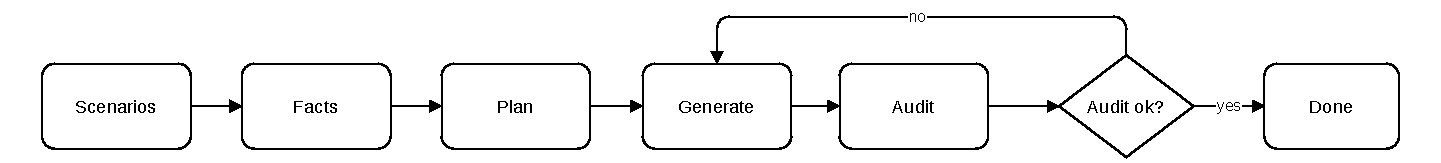
\includegraphics[width=\textwidth]{images/generation_pipeline.pdf}
    \caption[Generation pipeline, sample regenerated on audit failure]{The generation pipeline. A sample that fails the audit stage is regenerated.}
    \label{fig:pipeline-stages}
\end{figure}

\subsection{Cost}
\label{subsec:pipeline-cost}

Table~\ref{tab:pipeline-cost} reports the cost of producing both datasets, at Claude's Batch API prices, which halve the standard per-token rate. Each stage's figure is the total cost across every \texttt{generate} and \texttt{audit} iteration needed to reach the final set of samples, rather than the cost of a single pass. The \texttt{plan} and \texttt{facts} stages are not included: \texttt{plan} calls no model, and \texttt{facts} generates 150 short requests in total, a negligible cost next to the other stages.

\begin{table}[H]
    \centering
    \small
    \setlength{\tabcolsep}{3.5pt}
    \begin{tabular}{@{}llrrrrr@{}}
        \toprule
        & & \multicolumn{4}{c}{\textbf{Tokens (millions)}} & \\
        \cmidrule(lr){3-6}
        \textbf{Stage} & \textbf{Model} & \textbf{Input} & \textbf{Output} & \textbf{Cache read} & \textbf{Cache write} & \textbf{Cost} \\
        \midrule
        \texttt{generate}, single-turn            & Claude Haiku 4.5 & 4.32 & 0.61 & 0.00 & 0.00 & \$3.68 \\
        \texttt{generate}, multi-turn              & Claude Haiku 4.5 & 2.02 & 0.45 & 0.00 & 0.00 & \$2.15 \\
        \texttt{generate}, multi-turn \texttt{adversarial} & Claude Sonnet 5  & 1.49 & 1.44 & 1.40 & 2.34 & \$8.68 \\
        \texttt{audit}, single-turn                & Claude Sonnet 5  & 1.27 & 0.50 & 4.37 & 1.24 & \$3.78 \\
        \texttt{audit}, multi-turn                 & Claude Sonnet 5  & 2.38 & 0.53 & 4.77 & 1.23 & \$5.01 \\
        \midrule
        \textbf{Total} & & \textbf{11.47} & \textbf{3.53} & \textbf{10.54} & \textbf{4.81} & \textbf{\$23.30} \\
        \bottomrule
    \end{tabular}
    \caption[Tokens and cost for the single-turn and multi-turn datasets]{Tokens and cost of the run that produced the single-turn and multi-turn datasets, at Claude's Batch API prices. Input counts only the uncached input tokens.}
    \label{tab:pipeline-cost}
\end{table}


\section{Baselines}
\label{sec:dataset-baselines}

\subsection{Text-Only Classifiers}
\label{subsec:text-only-baselines}

Section~\ref{subsec:lexical-separability} requires the dataset to be difficult for classifiers that take only the request text as input, and it names three text representations that these classifiers must be trained on:

\begin{itemize}
    \item \textbf{bag-of-words}: a logistic regression over raw word counts (unigrams and bigrams);
    \item \textbf{TF-IDF}: a logistic regression over the same counts, weighted by TF-IDF;
    \item \textbf{sentence embeddings}: a logistic regression over sentence embeddings.
\end{itemize}

For each classifier, \emph{accuracy} is measured, given by
\begin{equation}
    \text{accuracy} = \frac{\text{requests classified correctly}}{\text{all requests}},
\end{equation}
where a request is classified correctly when the classifier's predicted sub-agent matches the correct sub-agent for that request.

Accuracy is measured with \emph{5-fold cross-validation}: the dataset is split into five folds, each classifier is trained on four folds and evaluated on the remaining fold, and this is repeated five times so that every fold serves once as the validation fold. Each fold, when it acts as the validation fold, produces a predicted sub-agent for every request in it. This is the \emph{out-of-fold prediction} for that request, since the request was never in the training data used to produce it. Collecting the out-of-fold prediction from each of the five folds gives one predicted sub-agent for every request in the dataset. Accuracy is then computed once, as defined above, by comparing each request's out-of-fold prediction against its correct sub-agent. This procedure uses every sample for both training and validation, without letting the same sample serve as both at once, and it prevents the reported accuracy from depending on one arbitrary split of the data. Folds are grouped by scenario, so a scenario's samples never split between the training fold and the validation fold. This matters for an \texttt{adversarial} pair, since its two requests share nearly all their wording: if one request were used for training and the other for validation, the classifier could match the validation request to its near-duplicate seen during training, and score high without learning to separate the sub-agents.

The sentence embeddings are obtained with \texttt{BAAI/bge-small-en-v1.5}, an embedding model that maps a request to a fixed-size vector encoding its meaning, so that requests with a similar meaning are mapped to nearby vectors.

Each classifier is trained and evaluated four times, on four different subsets of the samples:

\begin{itemize}
    \item \textbf{All}: the whole dataset;
    \item \textbf{Plain}: only the \texttt{plain} tier;
    \item \textbf{Natural}: only the \texttt{natural} tier;
    \item \textbf{Adversarial}: only the \texttt{adversarial} tier.
\end{itemize}

The accuracy obtained on both the single-turn and the multi-turn dataset is reported in Table~\ref{tab:text-baselines}.

\begin{table}[h]
    \centering
    \begin{tabular}{@{}l|lll|lll@{}}
        \toprule
        & \multicolumn{3}{c|}{\textbf{Single-turn}} & \multicolumn{3}{c}{\textbf{Multi-turn}} \\
        \textbf{Tier} & \textbf{Bag-of-words} & \textbf{TF-IDF} & \textbf{Embedding} & \textbf{Bag-of-words} & \textbf{TF-IDF} & \textbf{Embedding} \\
        \midrule
        Plain       & 0.900 & 0.993 & 0.927 & 0.840 & 0.987 & 0.873 \\
        Natural     & 0.708 & 0.730 & 0.653 & 0.665 & 0.677 & 0.592 \\
        Adversarial & 0.631 & 0.566 & 0.478 & 0.599 & 0.508 & 0.411 \\
        \midrule
        All         & 0.684 & 0.664 & 0.582 & 0.645 & 0.613 & 0.519 \\
        \bottomrule
    \end{tabular}
    \caption[Text-only classifier accuracy by difficulty tier, both datasets]{Accuracy of the three text-only classifiers, per difficulty tier, on the single-turn and the multi-turn dataset.}
    \label{tab:text-baselines}
\end{table}

On the whole dataset, no classifier reaches an accuracy above 0.69, on either the single-turn or the multi-turn dataset. Broken down by tier, accuracy falls from \texttt{plain} to \texttt{natural} and falls again from \texttt{natural} to \texttt{adversarial}, for all three classifiers, on both datasets. This is the decreasing accuracy that the tiers are designed to produce (Section~\ref{subsec:difficulty-tiers}). On \texttt{plain}, the request states only the binding constraint, so its vocabulary alone gives away the correct sub-agent. On \texttt{natural}, the request also states a waived constraint, so the vocabulary of a second sub-agent appears in the same request. On \texttt{adversarial}, the request is one half of a pair that shares nearly all its wording with its twin, so the words alone cannot tell which of the two constraints is binding.

The intrinsic difficulty of the \texttt{adversarial} design is also confirmed by the TF-IDF classifier results, which are outperformed by a non-TF-IDF-weighted bag-of-words classifier only on that tier, on both datasets. The two requests in an adversarial pair share nearly all their wording, and this high overlap makes TF-IDF down-weight words that still carry part of the routing signal.

The embedding classifier beats bag-of-words only on the \texttt{plain} tier. On \texttt{plain}, the request states one constraint, and the embedding captures it directly. On \texttt{natural}, the request also states a second, waived constraint. On \texttt{adversarial}, the request is nearly identical to its pair. In both cases, the embedding represents the whole request, and most of the request is the shared scenario text rather than the constraint that decides the sub-agent. Two requests built from the same scenario can then end up with similar embeddings even when they belong to different sub-agents, which lowers accuracy.

\subsection{Vocabulary and Routability}
\label{subsec:baseline-vocabulary}

Table~\ref{tab:baseline-terms} shows the single-turn TF-IDF terms with the highest weight, for each sub-agent. This confirms that most of the accuracy on \texttt{natural} and \texttt{adversarial} comes from requirement-specific vocabulary.

\begin{table}[h]
    \centering
    \begin{tabular}{@{}ll@{}}
        \toprule
        \textbf{Sub-agent} & \textbf{Highest-weighted TF-IDF terms} \\
        \midrule
        \texttt{legacy\_compat}     & contract, API, clients, existing, without breaking, published \\
        \texttt{time\_to\_market}       & weeks, working, demo, two weeks, ship, product \\
        \texttt{resource\_opt}      & memory, budget, ceiling, CPU, cloud, under \\
        \texttt{scale\_arch}        & scale, infrastructure, shared, horizontally, decouple, across \\
        \texttt{strict\_compliance} & audit, data, compliance, logging, security, officer \\
        \bottomrule
    \end{tabular}
    \caption[Highest-weighted TF-IDF terms per sub-agent]{Highest-weighted TF-IDF terms per sub-agent.}
    \label{tab:baseline-terms}
\end{table}

Section~\ref{subsec:lexical-separability} requires every request to stay routable to one sub-agent and to read as natural. The text-only baseline accuracies in Table~\ref{tab:text-baselines} are the lowest achievable under that requirement. To lower this accuracy further, the highest-weighted terms in Table~\ref{tab:baseline-terms} could be banned from generation, so that the generator cannot rely on them. The result is that the generator relies on synonyms instead, and a synonym is equally separable for a classifier. Banning every synonym as well introduces ambiguity: requests stop reading as natural and become hard to route even for a human.

\subsection{Difficulty Beyond the Baselines}
\label{subsec:encoder-robustness}

The generation pipeline is designed to minimize the accuracy of the three baselines whose results are reported in Table~\ref{tab:text-baselines}. Their low accuracy therefore does not show that the datasets are also difficult for other text-only classifiers. To show this, two more logistic regressions are trained on the representations of two different encoders, on the same scenario-grouped folds (Table~\ref{tab:modernbert-baseline}).

\begin{table}[H]
    \centering
    \small
    \begin{tabular}{@{}l|cc|cc@{}}
        \toprule
        & \multicolumn{2}{c|}{\textbf{Single-turn}} & \multicolumn{2}{c}{\textbf{Multi-turn}} \\
        \textbf{Tier} & \textbf{ModernBERT} & \textbf{BGE-M3} & \textbf{ModernBERT} & \textbf{BGE-M3} \\
        \midrule
        Plain       & 0.827 & 0.967 & 0.747 & 0.940 \\
        Natural     & 0.665 & 0.770 & 0.607 & 0.643 \\
        Adversarial & 0.552 & 0.524 & 0.462 & 0.431 \\
        \midrule
        All         & 0.618 & 0.654 & 0.541 & 0.555 \\
        \bottomrule
    \end{tabular}
    \caption[ModernBERT-large and BGE-M3 accuracy by difficulty tier]{Accuracy of the logistic regressions over ModernBERT-large representations and over BGE-M3 sentence embeddings, per difficulty tier, on the single-turn and the multi-turn dataset.}
    \label{tab:modernbert-baseline}
\end{table}

The first is trained on the representations of ModernBERT-large \cite{warnerSmarterBetterFaster2024}. ModernBERT-large maps each token of the request to a vector, and the representation of the request is obtained by mean pooling these vectors. The second is trained on the sentence embeddings of \texttt{BAAI/bge-m3}, a larger embedding model than \texttt{BAAI/bge-small-en-v1.5}.

Neither classifier reaches an accuracy above 0.69 on the whole dataset, single-turn or multi-turn, and the accuracy of both falls from \texttt{plain} to \texttt{natural} to \texttt{adversarial}, as for the three baselines. The difficulty is therefore a property of the datasets and is not specific to the three classifiers chosen as baselines.


\section{Statistical Analysis of Surface Features}
\label{sec:statistical-validation}

Section~\ref{subsec:lexical-separability} requires the sample set to be balanced across sub-agents in writing style, punctuation, and sentence pattern, not only in vocabulary. Without that balance, a text-only classifier could route a request by a stylistic marker instead of by what the request asks. This section reports an analysis of variance (ANOVA) that tests whether the dataset meets that requirement, over measurable \emph{surface features} of the request text, properties that define how a request is written, such as its length or its punctuation, computed directly from the characters and words of the request text.

\subsection{Design Factors}
\label{subsec:design-factors}

Every test in this section reads one or more of the following design factors:

\begin{itemize}
    \item \texttt{gold}: the correct sub-agent the request should be routed to.
    \item \texttt{decoy}: the sub-agent whose constraint is stated but waived, defined only when the sample carries a decoy.
    \item \texttt{difficulty}: the difficulty tier the sample was built at, \texttt{plain}, \texttt{natural}, or \texttt{adversarial} (Section~\ref{subsec:difficulty-tiers}).
    \item \texttt{pattern}: the decoy pattern used to write the adversarial pair, defined only for the \texttt{adversarial} tier (Section~\ref{subsec:difficulty-tiers}).
    \item \texttt{persona}: the writing style used to generate the request (Section~\ref{subsec:personas}).
\end{itemize}

\subsection{Sample Balance}
\label{subsec:sample-balance}

ANOVA assumes \emph{homoscedasticity}, that is, that the variance of the tested feature is the same in every group the factors define. Section~\ref{subsubsec:levene-kruskal} tests this assumption directly and finds it violated for several features. The F-test that ANOVA relies on is expected to remain robust to unequal variance when the design is balanced, that is, when every group holds the same number of samples \citep{glassConsequencesFailureMeet1972}.
This robustness is why the balance checked in this section matters beyond precision: it is also what keeps every ANOVA in this chapter valid despite the violated homoscedasticity assumption.

An unbalanced design also risks a different problem: an ANOVA can attribute variance to a factor that only occurs more often for one sub-agent, rather than to a real effect of that factor. The plan stage provides balanced samples by design (Section~\ref{subsec:pipeline-plan}), and Figure~\ref{fig:sample-balance} plots the sample counts that result.

\begin{figure}[H]
    \centering
    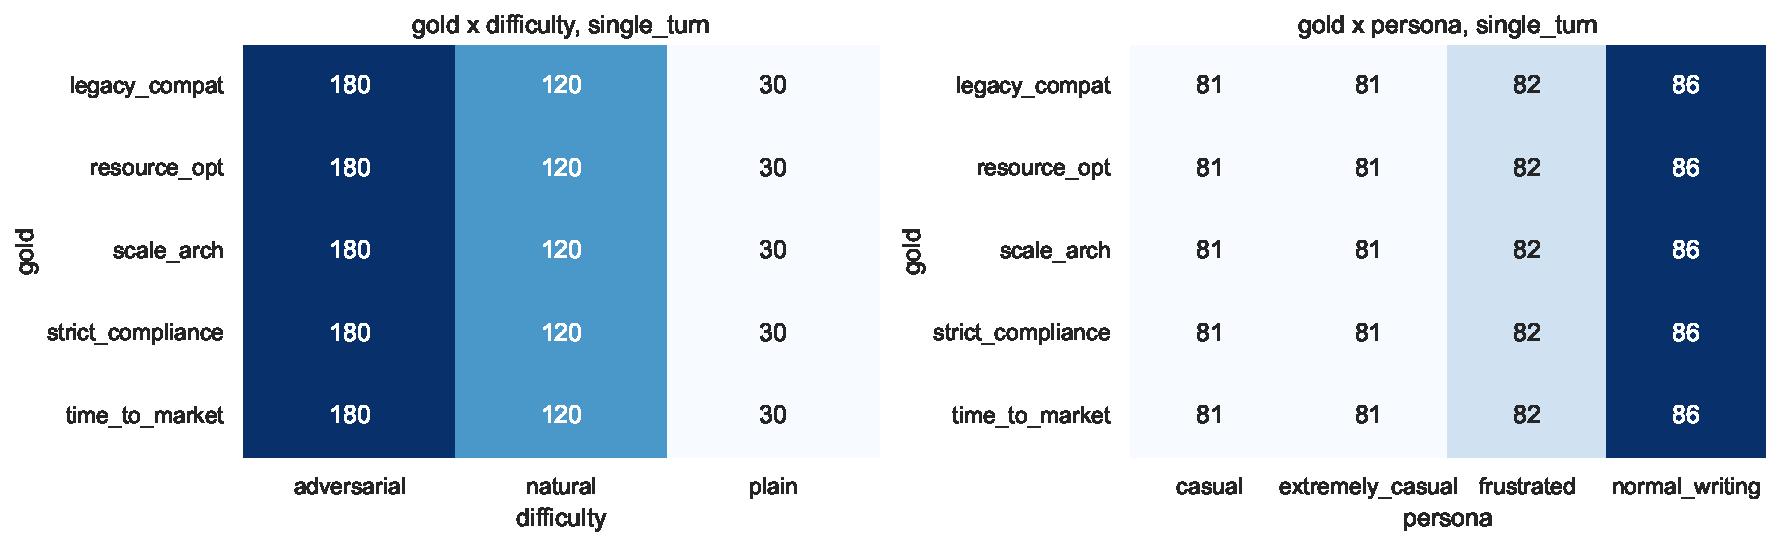
\includegraphics[width=\textwidth]{images/plots/anova/dataset_composition_single_turn.pdf}
    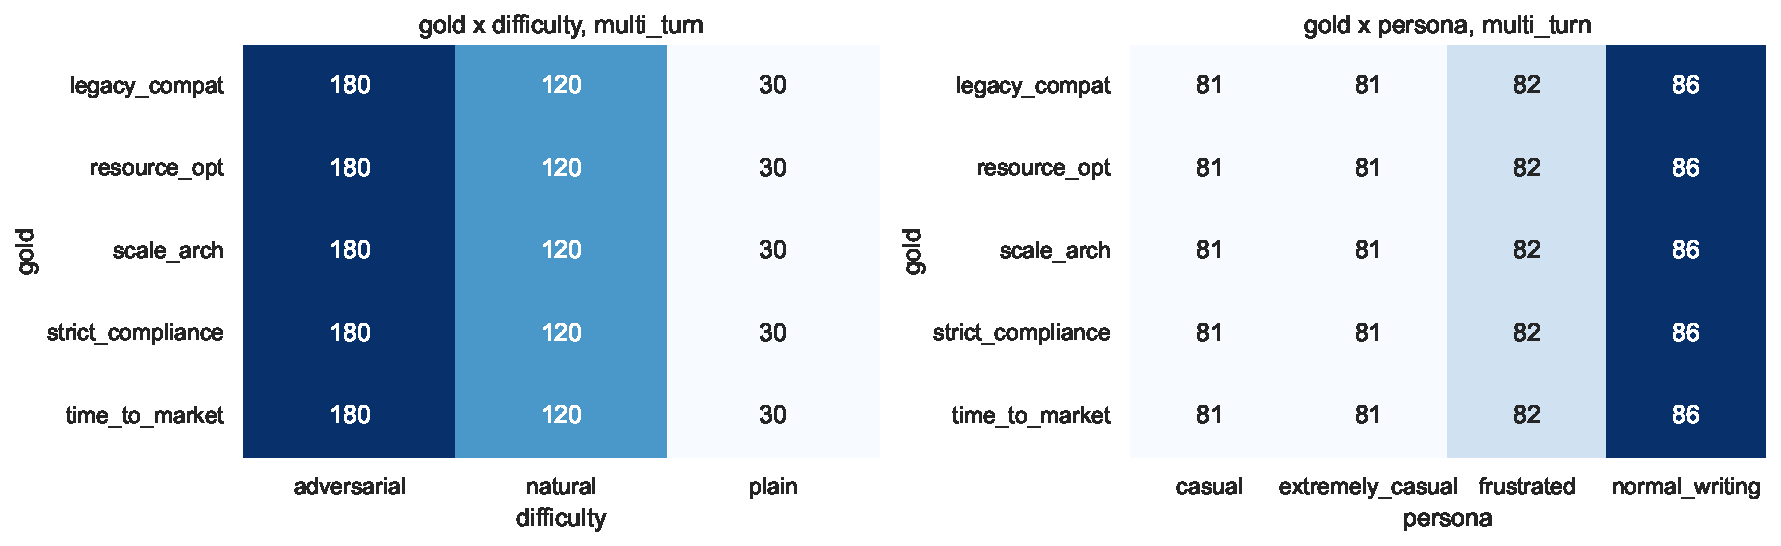
\includegraphics[width=\textwidth]{images/plots/anova/dataset_composition_multi_turn.pdf}
    \caption[Sample counts per sub-agent by tier and persona]{Sample counts per sub-agent, against difficulty tier and persona, single-turn (top) and multi-turn (bottom).}
    \label{fig:sample-balance}
\end{figure}

Figure~\ref{fig:sample-balance} cross-tabulates the correct sub-agent (\texttt{gold}) against the difficulty tier and against the persona, for the single-turn and the multi-turn dataset. Every sub-agent receives the same number of samples at every difficulty tier. Persona counts are near-equal but not identical across sub-agents, for example 81, 81, 82, and 86 samples for the four personas of a given sub-agent, because the deterministic shuffle in Section~\ref{subsec:pipeline-plan} distributes personas evenly only up to the remainder left when the sample count for a sub-agent is not a multiple of four. This gap, at most 5 samples out of about 330 per sub-agent, is negligible and does not compromise the balance that the tests in this section rely on.

\subsection{Extracted Features}
\label{subsec:surface-features}

The ANOVA in this section asks whether the correct sub-agent, \texttt{gold}, leaves a mark on the surface style of the request text, independent of its content. Section~\ref{sec:statistical-validation} requires the five sub-agents to be balanced in style: without that balance, a text-only classifier could route a request by a stylistic cue instead of by what the request asks. For each surface feature tested, the null hypothesis states that \texttt{gold} has no effect on it, that is, that the mean value of the feature is the same across the five sub-agent groups. Rejecting the null hypothesis for a feature means the sub-agent groups differ on that stylistic property.

For the ANOVA analysis, thirteen surface features are extracted from the text of each request. They are listed in Table~\ref{tab:surface-features}.

\begin{table}[H]
    \centering
    \begin{tabularx}{\textwidth}{@{}l>{\raggedright\arraybackslash}X@{}}
        \toprule
        \textbf{Feature} & \textbf{Definition} \\
        \midrule
        \texttt{n\_chars} & Number of characters \\
        \texttt{n\_words} & Number of words \\
        \texttt{n\_sentences} & Number of sentences \\
        \texttt{mean\_word\_len} & Mean word length, in characters \\
        \texttt{mean\_sent\_len} & Mean sentence length, in words \\
        \texttt{ttr} & Type-token ratio, distinct words divided by total words \\
        \texttt{pct\_upper} & Percentage of characters that are uppercase \\
        \texttt{pct\_digit} & Percentage of characters that are digits \\
        \texttt{n\_question} & Number of question marks \\
        \texttt{n\_comma} & Number of commas \\
        \texttt{long\_word\_ratio} & Percentage of words longer than seven characters \\
        \texttt{n\_units} & Count of unit and magnitude markers (\texttt{\%}, \texttt{\$}, MB, ms, req/s, and similar) \\
        \texttt{n\_number\_words} & Count of numbers written as words (\textit{eighty}, \textit{two weeks}, \textit{percent}) \\
        \bottomrule
    \end{tabularx}
    \caption[The thirteen surface features extracted from each request]{The thirteen surface features extracted from each request.}
    \label{tab:surface-features}
\end{table}

\subsection{One-Way ANOVA}
\label{subsec:anova-oneway}

For each of the thirteen surface features, a \emph{one-way ANOVA}, an ANOVA that tests one factor at a time, tests whether \texttt{gold} has an effect on that feature, for example whether the number of words in a request differs depending on which sub-agent is correct for it. Two quantities are reported for each test.

\paragraph{Effect size ($\omega^2$).} Omega squared is the percentage of the total variance in the feature explained by \texttt{gold}, corrected for the sampling noise that a simpler estimate (eta squared) would count as effect \citep{olejnikGeneralizedEtaOmega2003}. Cohen defines conventional thresholds for eta squared at 0.01 as small, 0.06 as medium, and 0.14 as large \citep{cohenStatisticalPowerAnalysis2013}; these thresholds are reused for omega squared as well.

\paragraph{Corrected significance ($p_{\text{holm}}$).} A one-way ANOVA returns a $p$-value for the null hypothesis that \texttt{gold} has no effect on a given feature. A raw $p$-value below 0.05 would count that effect as significant on its own. But thirteen tests are run at once, one per feature, and some of them are expected to fall below 0.05 purely by chance, even if \texttt{gold} has no real effect on any feature. The Holm method \citep{holmSimpleSequentiallyRejective1979} corrects for this. It raises the threshold each test must clear as more tests are run, and the corrected $p$-value is reported as $p_{\text{holm}}$. An effect counts as significant only when $p_{\text{holm}}$ stays below 0.05.

\bigskip

\begin{table}[htbp]
    \centering
    \small
    \begin{tabular}{@{}lrrrr@{}}
        \toprule
        & \multicolumn{2}{c}{\textbf{Single-turn}} & \multicolumn{2}{c}{\textbf{Multi-turn}} \\
        \textbf{Feature} & $\omega^2$ & $p_{\text{holm}}$ & $\omega^2$ & $p_{\text{holm}}$ \\
        \midrule
        \texttt{pct\_digit}        & \cellcolor{omegaMedium}0.132 & \textbf{$<$0.001} & \cellcolor{omegaMedium}0.082 & \textbf{$<$0.001} \\
        \texttt{n\_units}          & \cellcolor{omegaMedium}0.119 & \textbf{$<$0.001} & \cellcolor{omegaMedium}0.090 & \textbf{$<$0.001} \\
        \texttt{mean\_word\_len}   & \cellcolor{omegaMedium}0.063 & \textbf{$<$0.001} & \cellcolor{omegaMedium}0.075 & \textbf{$<$0.001} \\
        \texttt{long\_word\_ratio} & \cellcolor{omegaMedium}0.062 & \textbf{$<$0.001} & \cellcolor{omegaSmall}0.046  & \textbf{$<$0.001} \\
        \texttt{n\_comma}          & \cellcolor{omegaSmall}0.036  & \textbf{$<$0.001} & \cellcolor{omegaSmall}0.016  & \textbf{$<$0.001} \\
        \texttt{n\_chars}          & \cellcolor{omegaSmall}0.024  & \textbf{$<$0.001} & \cellcolor{omegaSmall}0.015  & \textbf{$<$0.001} \\
        \texttt{n\_words}          & \cellcolor{omegaSmall}0.016  & \textbf{$<$0.001} & 0.006 & \textbf{0.038} \\
        \texttt{n\_number\_words}  & \cellcolor{omegaSmall}0.015  & \textbf{$<$0.001} & \cellcolor{omegaSmall}0.011  & \textbf{0.002} \\
        \texttt{ttr}               & \cellcolor{omegaSmall}0.014  & \textbf{$<$0.001} & \cellcolor{omegaSmall}0.011  & \textbf{0.002} \\
        \texttt{pct\_upper}        & \cellcolor{omegaSmall}0.013  & \textbf{$<$0.001} & 0.003 & 0.242 \\
        \texttt{mean\_sent\_len}   & 0.004 & 0.120 & -0.001 & 1.000 \\
        \texttt{n\_sentences}      & 0.001 & 0.374 & -0.001 & 1.000 \\
        \texttt{n\_question}       & -0.002 & 0.914 & -0.001 & 1.000 \\
        \bottomrule
    \end{tabular}
    \caption[Effect of \texttt{gold} on surface features, single-turn and multi-turn]{Effect of \texttt{gold} on the thirteen surface features, single-turn and multi-turn.}
    \label{tab:gold-omega2}
\end{table}

Table~\ref{tab:gold-omega2} reports the effect of \texttt{gold} on all thirteen features, ordered by $\omega^2$: cells are shaded by magnitude, \colorbox{omegaSmall}{small}, \colorbox{omegaMedium}{medium}, \colorbox{omegaLarge}{large}, and left unshaded when negligible, and $p_{\text{holm}}$ is bold where it rejects the null hypothesis. The largest effect of \texttt{gold} falls on the count of numeric magnitudes, \texttt{pct\_digit} and \texttt{n\_units} at 0.132 and 0.119 in single-turn, 0.082 and 0.090 in multi-turn. When the correct sub-agent is \texttt{resource\_opt}, the request is more likely to state memory ceilings, cost budgets, or latency figures. Figure~\ref{fig:gold-effect} shows this difference directly, plotting the group means of \texttt{pct\_digit} and \texttt{n\_units} with a 95\% confidence interval per sub-agent, single-turn (top) and multi-turn (bottom).

\begin{figure}[htbp]
    \centering
    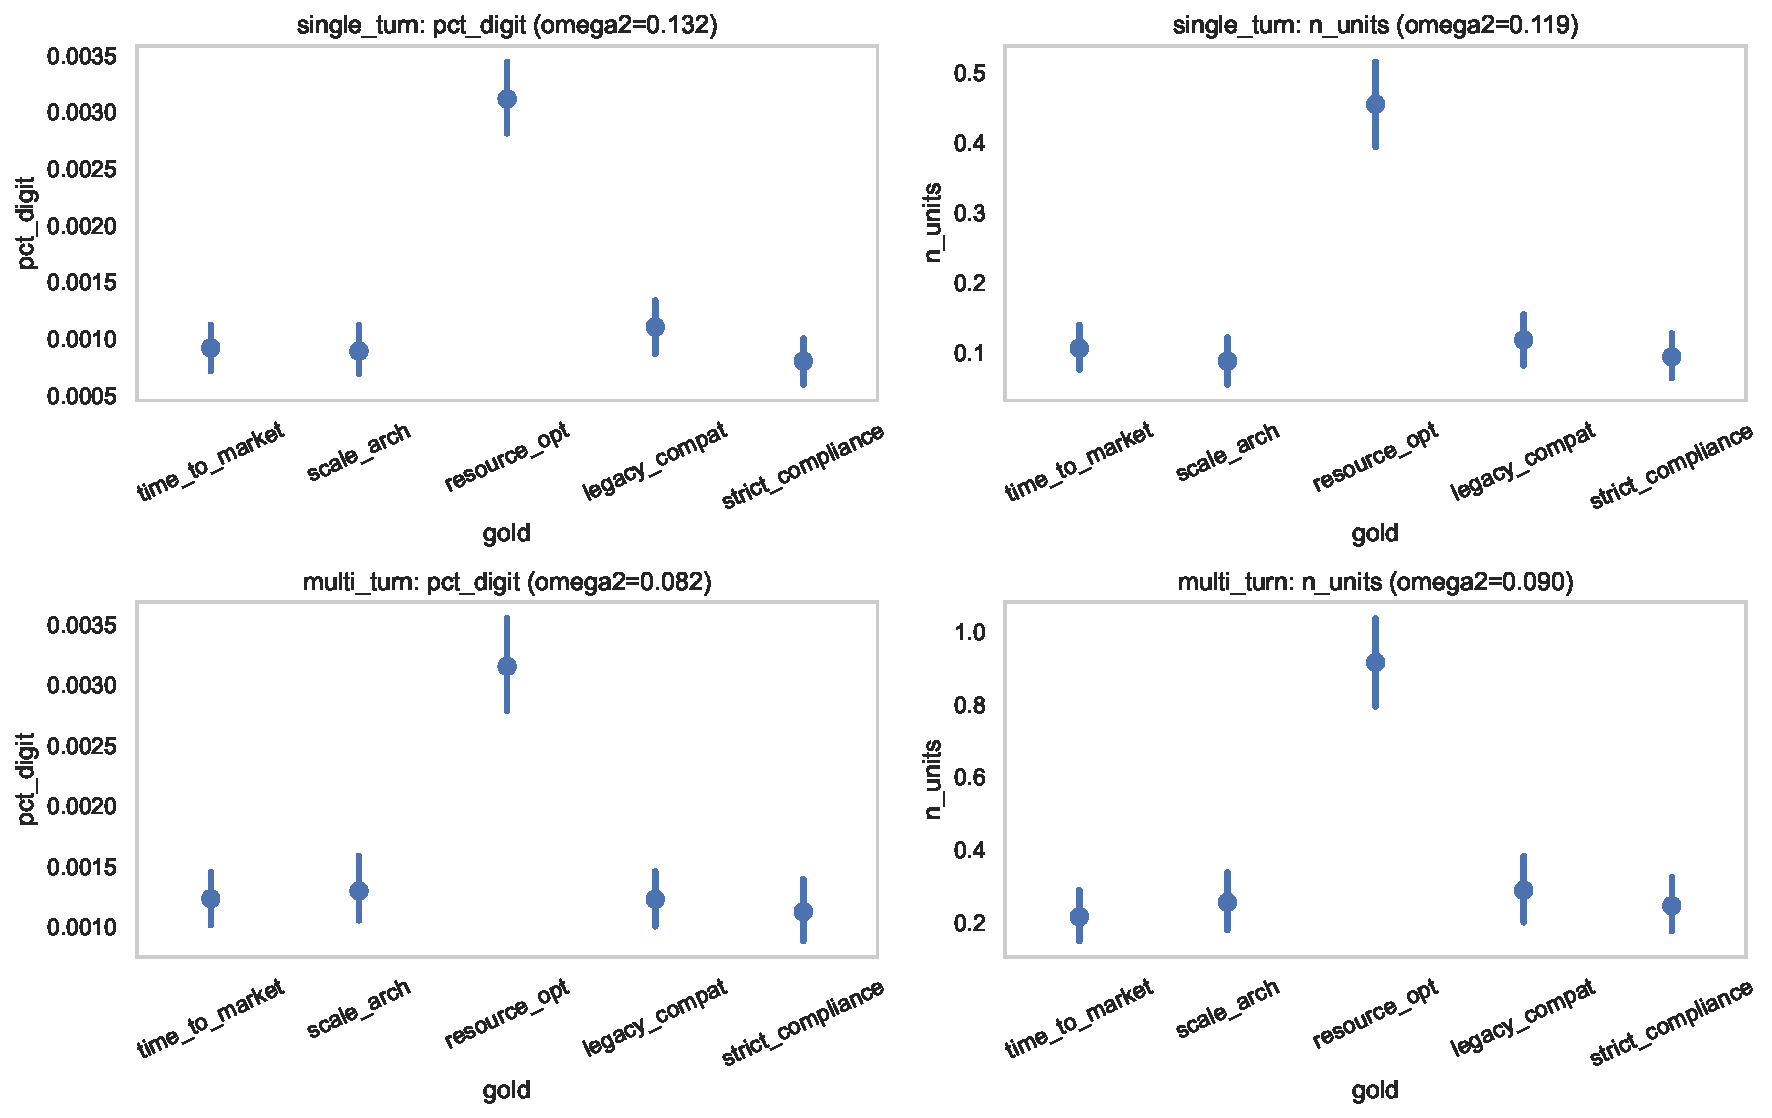
\includegraphics[width=\textwidth]{images/plots/anova/dataset_gold.pdf}
    \caption[Group means of \texttt{pct\_digit} and \texttt{n\_units} by \texttt{gold}]{Group means of \texttt{pct\_digit} and \texttt{n\_units} by \texttt{gold}, single-turn (top) and multi-turn (bottom).}
    \label{fig:gold-effect}
\end{figure}

\subsection{Levene's Test and the Kruskal-Wallis Test}
\label{subsubsec:levene-kruskal}

The one-way ANOVA in Section~\ref{subsec:anova-oneway} is valid only if the five \texttt{gold} groups share the same variance. If this assumption fails for a feature, the ANOVA's $p$-value for that feature cannot be trusted, and the effect it reports could be a product of unequal variance rather than a real difference between the groups. Two additional tests check this assumption and its consequences:

\begin{itemize}
    \item \textbf{Levene}'s test checks directly whether the five groups have equal variance, the assumption the ANOVA needs \citep{montgomeryDesignAnalysisExperiments2022}.
    \item The \textbf{Kruskal-Wallis} test \citep{montgomeryDesignAnalysisExperiments2022} compares the same \texttt{gold} groups on the ranks of the values instead of the raw values. This comparison needs no assumption about variance, so it stays valid even on a feature where Levene shows the ANOVA's assumption fails, and its verdict serves as a check on the ANOVA's own verdict for that feature.
\end{itemize}

Table~\ref{tab:levene-kruskal} reports both tests on the same thirteen features and the same \texttt{gold} factor as Table~\ref{tab:gold-omega2}, with both $p$-values corrected with Holm across that same family of thirteen tests. Bold marks a $p_{\text{holm}}$ below 0.05, rejecting the test's null hypothesis.

\begin{table}[htbp]
    \centering
    \small
    \begin{tabular}{@{}lrrrr@{}}
        \toprule
        & \multicolumn{2}{c}{\textbf{Single-turn}} & \multicolumn{2}{c}{\textbf{Multi-turn}} \\
        \textbf{Feature} & \textbf{Levene} $p_{\text{holm}}$ & \textbf{Kruskal} $p_{\text{holm}}$ & \textbf{Levene} $p_{\text{holm}}$ & \textbf{Kruskal} $p_{\text{holm}}$ \\
        \midrule
        \texttt{pct\_digit}        & \textbf{$<$0.001} & \textbf{$<$0.001} & \textbf{$<$0.001} & \textbf{$<$0.001} \\
        \texttt{n\_units}          & \textbf{$<$0.001} & \textbf{$<$0.001} & \textbf{$<$0.001} & \textbf{$<$0.001} \\
        \texttt{mean\_word\_len}   & 1.000          & \textbf{$<$0.001} & 1.000          & \textbf{$<$0.001} \\
        \texttt{long\_word\_ratio} & 0.654          & \textbf{$<$0.001} & 1.000          & \textbf{$<$0.001} \\
        \texttt{n\_comma}          & \textbf{0.002} & \textbf{$<$0.001} & 1.000          & \textbf{$<$0.001} \\
        \texttt{n\_chars}          & \textbf{0.009} & \textbf{$<$0.001} & 1.000          & \textbf{$<$0.001} \\
        \texttt{n\_words}          & \textbf{0.048} & \textbf{0.002} & 1.000          & \textbf{0.034} \\
        \texttt{n\_number\_words}  & 0.364          & \textbf{$<$0.001} & 0.555          & \textbf{0.001} \\
        \texttt{ttr}               & 0.504          & \textbf{$<$0.001} & 1.000          & \textbf{0.001} \\
        \texttt{pct\_upper}        & \textbf{$<$0.001} & \textbf{0.004} & \textbf{$<$0.001} & 0.282          \\
        \texttt{mean\_sent\_len}   & 1.000          & \textbf{0.047} & 1.000          & 1.000          \\
        \texttt{n\_sentences}      & 0.271          & 0.426          & 1.000          & 1.000          \\
        \texttt{n\_question}       & 1.000          & 0.929          & 1.000          & 1.000          \\
        \bottomrule
    \end{tabular}
    \caption[Levene and Kruskal-Wallis tests on \texttt{gold}, single-turn and multi-turn]{Levene's test and the Kruskal-Wallis test on the \texttt{gold} factor, single-turn and multi-turn.}
    \label{tab:levene-kruskal}
\end{table}

\textbf{Levene}'s test rejects equal variance on six features in the single-turn dataset (\texttt{pct\_digit}, \texttt{n\_units}, \texttt{n\_comma}, \texttt{n\_chars}, \texttt{n\_words}, \texttt{pct\_upper}) and three in the multi-turn dataset (\texttt{pct\_digit}, \texttt{n\_units}, \texttt{pct\_upper}). The ANOVA's equal-variance assumption therefore does not hold for these features.

The \textbf{Kruskal-Wallis} test reaches the same verdict as the ANOVA on twelve of the thirteen features in the single-turn dataset and on all thirteen in the multi-turn dataset. The one exception is \texttt{mean\_sent\_len} in single-turn: the ANOVA does not reject its null hypothesis ($p_{\text{holm}} = 0.120$), but the Kruskal-Wallis test does ($p_{\text{holm}} = 0.047$). This feature has the smallest effect size in Table~\ref{tab:gold-omega2} ($\omega^2 = 0.004$), and both raw $p$-values are close to 0.05 before correction ($p = 0.040$ for the ANOVA, $p = 0.016$ for Kruskal-Wallis). After Holm's correction, one is above 0.05 and the other is below it. Levene's test does not reject equal variance for this feature ($p_{\text{holm}} = 1.000$), so the disagreement is not caused by a violated assumption.

Levene's test shows that the ANOVA's equal-variance assumption fails for a minority of features, six in single-turn and three in multi-turn. Despite this, the Kruskal-Wallis test agrees with the ANOVA on every feature but one, even though it needs no such assumption. The $\omega^2$ values in Table~\ref{tab:gold-omega2} therefore describe a property of the data, not an artifact of the ANOVA's violated assumption.

\subsection{Games-Howell Test}
\label{subsec:anova-posthoc}

The one-way ANOVA does not identify which pairs of sub-agents differ on a feature. To test this, a Games-Howell test is performed on every feature whose one-way \texttt{gold} effect stays significant after the Holm correction and reaches an $\omega^2$ of at least 0.01, the conventional threshold for a small effect.

The Games-Howell test compares every pair of sub-agents on a feature, all ten pairs at once, and holds the probability of at least one false positive among them at 0.05. Unlike Tukey's HSD test \citep{montgomeryDesignAnalysisExperiments2022}, it does not assume equal variances across groups \citep{gamesPairwiseMultipleComparison1976}, so it applies directly to the features where Section~\ref{subsubsec:levene-kruskal} shows this assumption fails.
After the Games-Howell test, the $p$-values from all pairwise comparisons are corrected with Holm across the restricted family of features.

Figure~\ref{fig:posthoc} shows the pairwise mean differences for the four features with the largest \texttt{gold} effect. A blank cell marks a pair that is not significant after the Holm correction.

\begin{figure}[htbp]
    \centering
    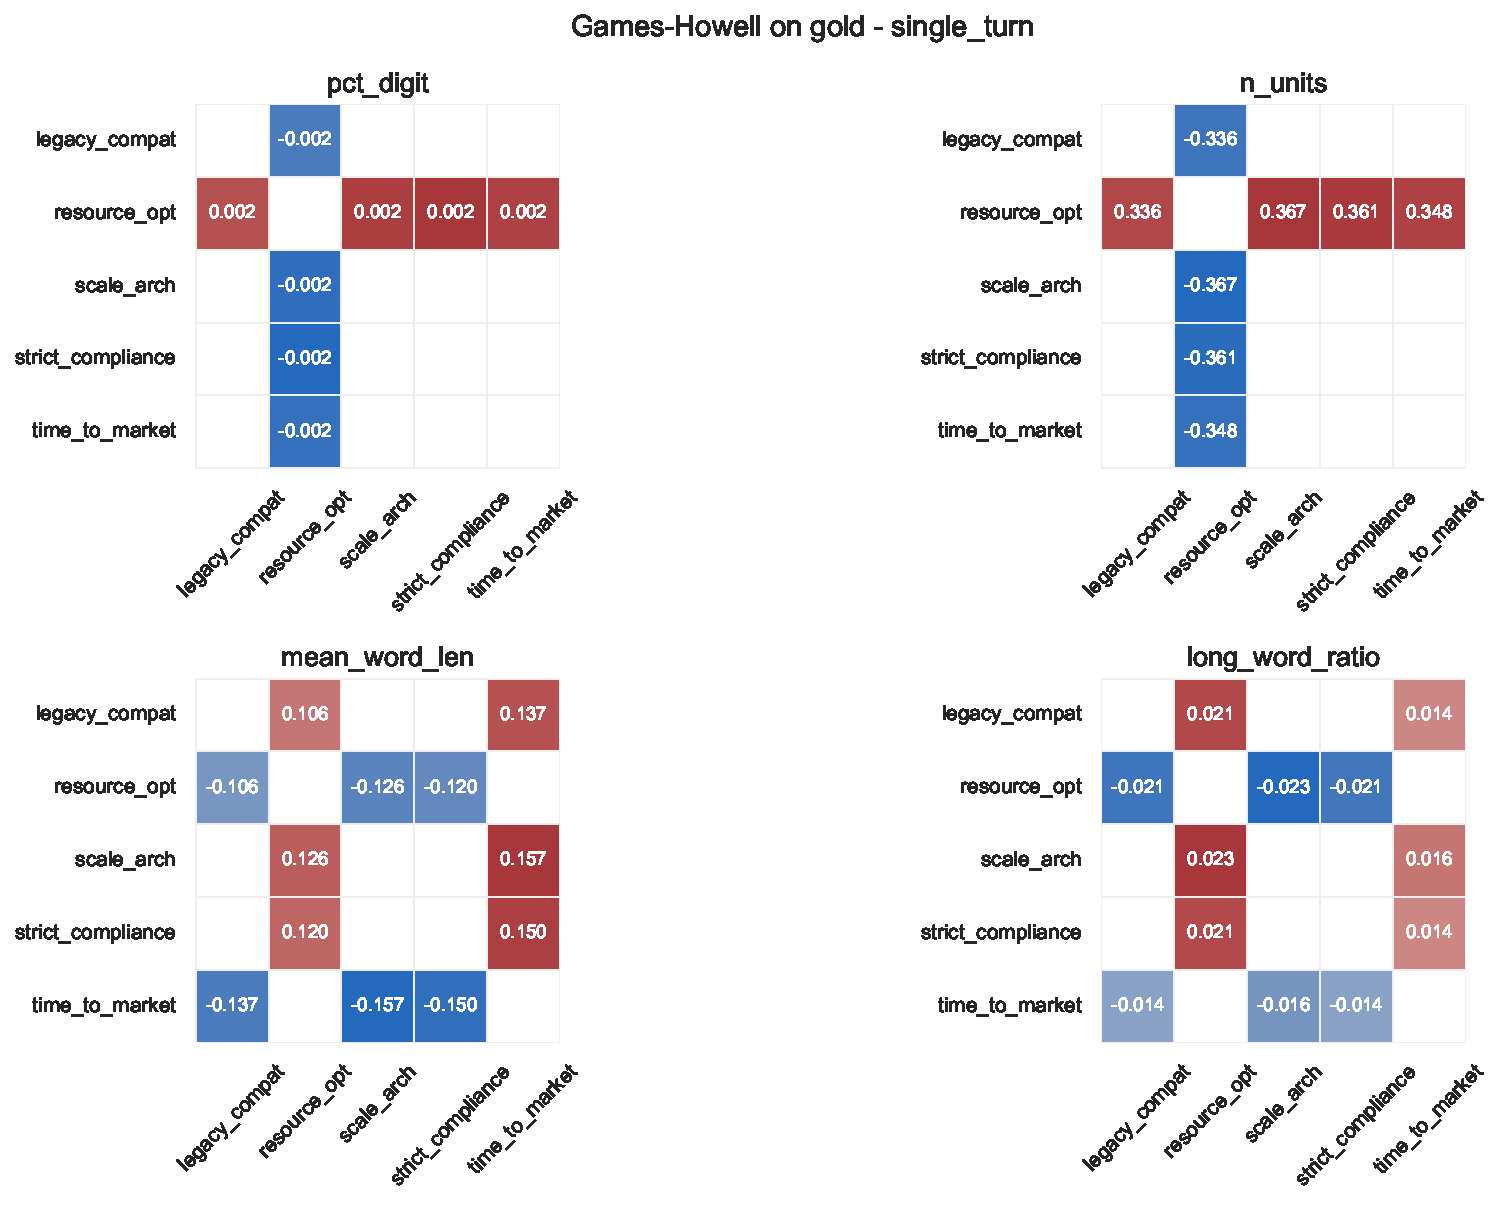
\includegraphics[width=\textwidth,height=0.46\textheight,keepaspectratio]{images/plots/anova/dataset_posthoc_single_turn.pdf}
    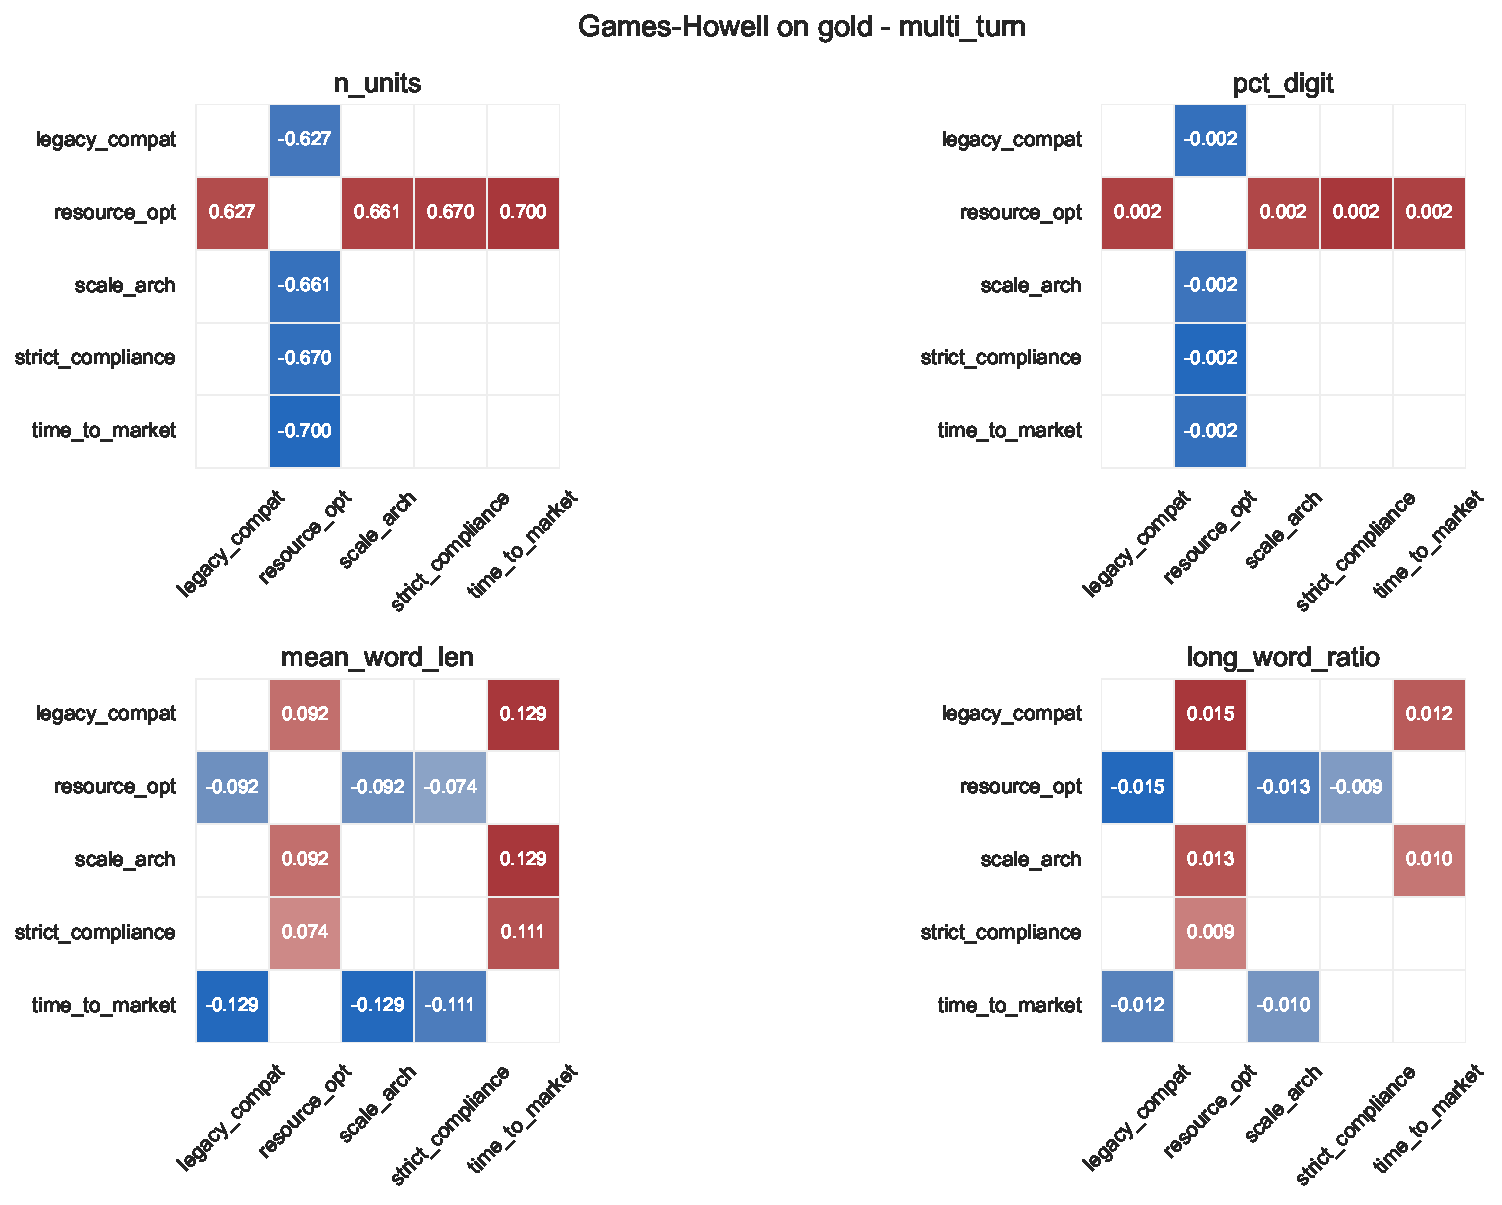
\includegraphics[width=\textwidth,height=0.46\textheight,keepaspectratio]{images/plots/anova/dataset_posthoc_multi_turn.pdf}
    \caption[Games-Howell pairwise comparisons on \texttt{gold} by dataset]{Games-Howell pairwise comparisons on \texttt{gold}, for the four surface features with the largest one-way effect, single-turn (top) and multi-turn (bottom) dataset. A blank cell means the pair is not significant after the Holm correction.}
    \label{fig:posthoc}
\end{figure}

The results on the single-turn dataset show the following structure:
\begin{itemize}
    \item On \texttt{pct\_digit} and \texttt{n\_units}, \texttt{resource\_opt} differs significantly from each of the other four sub-agents. None of the six pairs among those other four is significant. These two features therefore separate \texttt{resource\_opt} from the rest, but do not separate the remaining four sub-agents from each other.
    \item On \texttt{mean\_word\_len} and \texttt{long\_word\_ratio}, the sub-agents split into two blocks: \texttt{time\_to\_market} and \texttt{resource\_opt} on one side, \texttt{scale\_arch}, \texttt{legacy\_compat}, and \texttt{strict\_compliance} on the other. Every pair across the two blocks is significant, and no pair inside either block is. This split reflects domain-specific vocabulary: terms such as \textit{compliance}, \textit{infrastructure}, and \textit{migration} run longer than terms such as \textit{ship}, \textit{weeks}, and \textit{quick}.
\end{itemize}

The results on the multi-turn dataset show the same structure, with one exception:
\begin{itemize}
    \item On \texttt{pct\_digit} and \texttt{n\_units}, \texttt{resource\_opt} again differs significantly from each of the other four sub-agents, with no significant pair among those four.
    \item On \texttt{mean\_word\_len}, the same two blocks reappear: every pair across the two blocks is significant, and no pair inside either block is. On \texttt{long\_word\_ratio}, the same holds for five of the six pairs across the two blocks. The sixth pair, \texttt{time\_to\_market} against \texttt{strict\_compliance}, is not significant, even though the two sub-agents fall on opposite blocks.
\end{itemize}

This test confirms the same distinction among the five sub-agents. On \texttt{pct\_digit} and \texttt{n\_units}, \texttt{resource\_opt} separates from the other four. On \texttt{mean\_word\_len} and \texttt{long\_word\_ratio}, the five sub-agents split into two vocabulary blocks.

The stylistic imbalance that the one-way ANOVA detects is therefore not spread evenly across the five sub-agents. It traces to two distinct sources: \texttt{resource\_opt} stated apart from the other four by its numeric magnitude markers, and a two-block split in word length that follows domain vocabulary rather than the five sub-agents individually. Neither source separates all five sub-agents from each other on any single feature.

\subsection{Multiway ANOVA}
\label{subsec:anova-multiway}

The one-way test in Section~\ref{subsec:anova-oneway} examines one factor at a time. A \emph{multiway ANOVA} tests several factors together, so that the effect of each factor is estimated while holding the others fixed, and can also test whether two factors interact, that is, whether the effect of one factor changes depending on the level of the other. If, for example, \texttt{resource\_opt} requests used longer words only when the decoy was \texttt{time\_to\_market}, and shorter words only when the decoy was \texttt{scale\_arch}, averaging over decoys would hide the effect entirely.

Each interaction effect is isolated by comparing two nested regressions: a \texttt{full} model containing every combination of the listed factors, and a \texttt{reduced} model containing the same factors without any combination involving \texttt{gold}. The variance that the full model explains beyond the reduced model is the variance attributable to \texttt{gold}'s interactions with the other factors in that model. This gain is reported as \textbf{partial omega squared} ($\omega_p^2$): the gain divided by the variance that the reduced model left unexplained. It is corrected the same way as the one-way $\omega^2$, but for the sampling noise of the extra columns that the full model adds, on the block of interaction terms rather than on a single term \citep{olejnikGeneralizedEtaOmega2003}. Each comparison is tested with an F-test between the two nested models, Holm-corrected across the 13 features of each model.

\raggedbottom

Three such model pairs test for interactions between \texttt{gold} and the other design factors.

\begin{itemize}
    \item \textbf{Model 1 (style):} \texttt{gold * difficulty * persona}, fit on all 1650 samples.
    \item \textbf{Model 2 (difficulty):} \texttt{gold * decoy * difficulty}, fit on the 1500 samples that carry a decoy.
    \item \textbf{Model 3 (pattern):} \texttt{gold * pattern}, fit on the 900 \texttt{adversarial} samples.
\end{itemize}

Tables~\ref{tab:interactions-single} and~\ref{tab:interactions-multi} report partial $\omega^2$ and $p_{\text{holm}}$ for every feature and every model, single-turn and multi-turn. As in Table~\ref{tab:gold-omega2}, cells are shaded by magnitude, \colorbox{omegaSmall}{small}, \colorbox{omegaMedium}{medium}, \colorbox{omegaLarge}{large}, and left unshaded when negligible, using the same 0.01/0.06/0.14 thresholds \citep{cohenStatisticalPowerAnalysis2013}, and $p_{\text{holm}}$ is bold where it rejects the null hypothesis. These thresholds were defined for the one-way case, and applying them to partial omega squared can overstate the effect \citep{olejnikGeneralizedEtaOmega2003}.

Across the 78 tests spanning the three models and both datasets, only two cells reject the null hypothesis after Holm in single-turn and three in multi-turn. Their partial $\omega^2$ stays between 0.018 and 0.030 in every case, close to the small-effect threshold rather than far above it, so the conclusion holds even if the thresholds overstate the effect as described above.

The multiway analysis therefore finds no interaction effect worth reporting beyond the one-way ANOVA in Section~\ref{subsec:anova-oneway}.

\begin{table}[H]
    \centering
    \small
    \begin{tabular}{@{}lrrrrrr@{}}
        \toprule
        & \multicolumn{2}{c}{\textbf{Model 1 (style)}} & \multicolumn{2}{c}{\textbf{Model 2 (difficulty)}} & \multicolumn{2}{c}{\textbf{Model 3 (pattern)}} \\
        \textbf{Feature} & $\omega_p^2$ & $p_{\text{holm}}$ & $\omega_p^2$ & $p_{\text{holm}}$ & $\omega_p^2$ & $p_{\text{holm}}$ \\
        \midrule
        \texttt{pct\_digit}        & -0.008 & 1.000 & -0.004 & 1.000 & -0.007 & 1.000 \\
        \texttt{n\_units}          & -0.000 & 1.000 & -0.005 & 1.000 & -0.010 & 1.000 \\
        \texttt{mean\_word\_len}   & -0.005 & 1.000 & -0.005 & 1.000 & -0.005 & 1.000 \\
        \texttt{long\_word\_ratio} & -0.003 & 1.000 & -0.008 & 1.000 & -0.003 & 1.000 \\
        \texttt{n\_comma}          & -0.002 & 1.000 & 0.004  & 1.000 & -0.002 & 1.000 \\
        \texttt{n\_chars}          & -0.001 & 1.000 & -0.000 & 1.000 & -0.000 & 1.000 \\
        \texttt{n\_words}          & -0.001 & 1.000 & 0.001  & 1.000 & -0.001 & 1.000 \\
        \texttt{n\_number\_words}  & -0.006 & 1.000 & -0.004 & 1.000 & 0.003  & 1.000 \\
        \texttt{ttr}               & 0.005  & 1.000 & -0.003 & 1.000 & 0.003  & 1.000 \\
        \texttt{pct\_upper}        & \cellcolor{omegaSmall}0.022  & \textbf{0.009} & -0.011 & 1.000 & -0.004 & 1.000 \\
        \texttt{mean\_sent\_len}   & -0.006 & 1.000 & 0.008  & 0.855 & -0.004 & 1.000 \\
        \texttt{n\_sentences}      & 0.011  & 0.490 & \cellcolor{omegaSmall}0.020  & \textbf{0.007} & 0.009  & 0.808 \\
        \texttt{n\_question}       & 0.009  & 0.867 & 0.006  & 1.000 & -0.006 & 1.000 \\
        \bottomrule
    \end{tabular}
    \caption[Partial $\omega^2$ of \texttt{gold} interaction terms, single-turn dataset]{Partial $\omega^2$ ($\omega_p^2$) of the \texttt{gold} interaction terms, single-turn dataset.}
    \label{tab:interactions-single}

    \vspace{3em}

    \begin{tabular}{@{}lrrrrrr@{}}
        \toprule
        & \multicolumn{2}{c}{\textbf{Model 1 (style)}} & \multicolumn{2}{c}{\textbf{Model 2 (difficulty)}} & \multicolumn{2}{c}{\textbf{Model 3 (pattern)}} \\
        \textbf{Feature} & $\omega_p^2$ & $p_{\text{holm}}$ & $\omega_p^2$ & $p_{\text{holm}}$ & $\omega_p^2$ & $p_{\text{holm}}$ \\
        \midrule
        \texttt{pct\_digit}        & \cellcolor{omegaSmall}0.018  & \textbf{0.045} & -0.005 & 1.000 & -0.007 & 1.000 \\
        \texttt{n\_units}          & 0.004  & 0.975 & 0.002  & 1.000 & -0.004 & 1.000 \\
        \texttt{mean\_word\_len}   & 0.010  & 0.585 & 0.010  & 0.397 & -0.000 & 1.000 \\
        \texttt{long\_word\_ratio} & 0.001  & 0.975 & 0.001  & 1.000 & 0.003  & 1.000 \\
        \texttt{n\_comma}          & -0.000 & 0.975 & 0.002  & 1.000 & 0.004  & 1.000 \\
        \texttt{n\_chars}          & 0.006  & 0.975 & 0.006  & 1.000 & -0.003 & 1.000 \\
        \texttt{n\_words}          & 0.006  & 0.975 & 0.005  & 1.000 & -0.003 & 1.000 \\
        \texttt{n\_number\_words}  & 0.006  & 0.975 & 0.005  & 1.000 & 0.006  & 1.000 \\
        \texttt{ttr}               & 0.003  & 0.975 & -0.008 & 1.000 & -0.002 & 1.000 \\
        \texttt{pct\_upper}        & \cellcolor{omegaSmall}0.030  & \textbf{$<$0.001} & -0.004 & 1.000 & -0.006 & 1.000 \\
        \texttt{mean\_sent\_len}   & 0.008  & 0.786 & 0.003  & 1.000 & -0.004 & 1.000 \\
        \texttt{n\_sentences}      & 0.007  & 0.913 & 0.010  & 0.390 & -0.002 & 1.000 \\
        \texttt{n\_question}       & \cellcolor{omegaSmall}0.019  & \textbf{0.025} & -0.004 & 1.000 & -0.004 & 1.000 \\
        \bottomrule
    \end{tabular}
    \caption[Partial $\omega^2$ of \texttt{gold} interaction terms, multi-turn dataset]{Partial $\omega^2$ ($\omega_p^2$) of the \texttt{gold} interaction terms, multi-turn dataset.}
    \label{tab:interactions-multi}
\end{table}

\flushbottom

\subsection{Classifiers on Surface Features Alone}
\label{subsec:shortcut-classifiers}

The one-way and multiway ANOVA are univariate. Several small effects could still combine into one effect that a classifier exploits. A classifier that is trained on the thirteen surface features, with no access to the request text, measures the accuracy that such a combination reaches.

Two classifiers are trained, both on the same scenario-grouped 5-fold cross-validation and the same out-of-fold accuracy, broken down by difficulty tier, as the text-only classifiers of Section~\ref{sec:dataset-baselines}:

\begin{itemize}
    \item \textbf{Logistic regression}, trained five times to isolate the contribution of the numeric features to the accuracy reached from surface features alone:
    \begin{itemize}
        \item on all thirteen features, to establish the maximum accuracy attainable from surface features alone;
        \item on the feature set without \texttt{pct\_digit}, to measure how much the percentage of digit characters contributes to accuracy;
        \item on \texttt{pct\_digit} alone, to measure that feature's own contribution;
        \item on the feature set without the numeric features (\texttt{pct\_digit}, \texttt{n\_units}, \texttt{n\_number\_words}), to measure how much digit characters, unit markers, and numbers written as words together contribute to accuracy;
        \item on the numeric features alone, to measure how much they increase classification accuracy by themselves.
    \end{itemize}
    \item \textbf{Random forest}, trained once, on all thirteen features. It gives a second, non-linear ceiling, and it is the classifier used for the feature importance attribution of Section~\ref{subsec:feature-importance}.
\end{itemize}

Figures~\ref{fig:ceiling-single} and~\ref{fig:ceiling-multi} report accuracy for each of the six runs above, with chance accuracy marked for comparison.

\begin{figure}[htbp]
    \centering
    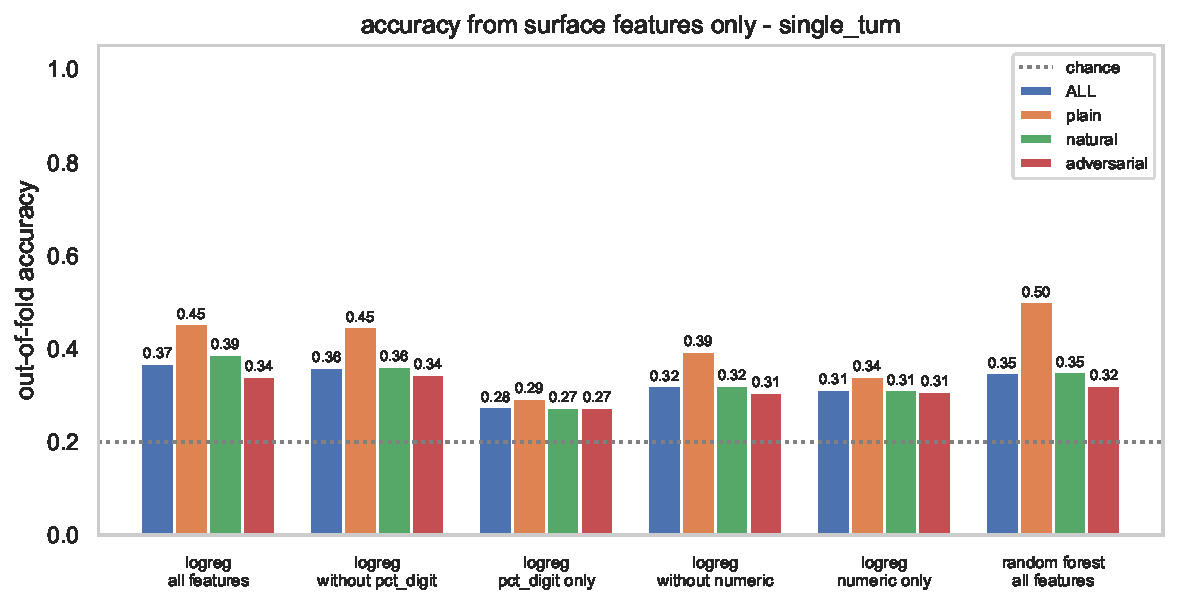
\includegraphics[width=\textwidth]{images/plots/anova/dataset_ceiling_single_turn.pdf}
    \caption[Accuracy from surface features alone, single-turn dataset]{Accuracy from surface features alone, single-turn dataset. The dotted line marks chance.}
    \label{fig:ceiling-single}
\end{figure}

\begin{figure}[htbp]
    \centering
    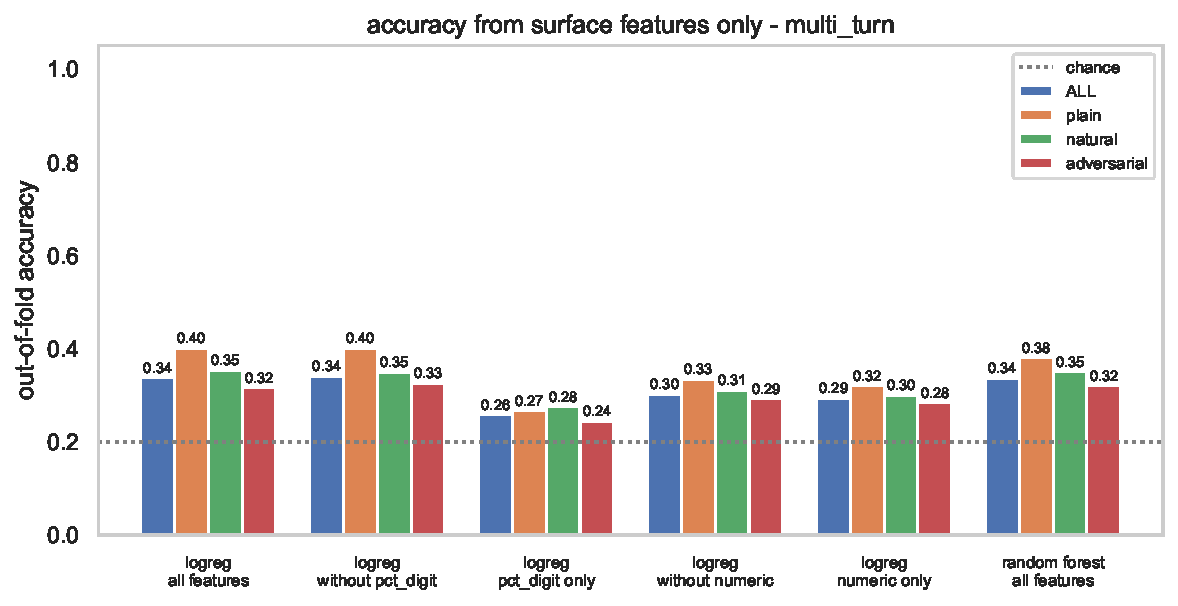
\includegraphics[width=\textwidth]{images/plots/anova/dataset_ceiling_multi_turn.pdf}
    \caption[Accuracy from surface features alone, multi-turn dataset]{Accuracy from surface features alone, multi-turn dataset. The dotted line marks chance.}
    \label{fig:ceiling-multi}
\end{figure}

Removing \texttt{pct\_digit} alone has a negligible effect on accuracy: 0.368 to 0.360 in single-turn and 0.337 to 0.341 in multi-turn. Removing all three numeric features instead costs a measurable amount of accuracy: from 0.368 to 0.320 in single-turn, and from 0.337 to 0.302 in multi-turn. The numeric features alone reach 0.313 in single-turn and 0.293 in multi-turn, nearly matching the 0.368 and 0.337 reached with all thirteen features. The other ten features therefore add only about 0.05 of accuracy beyond the numeric features. This shows that the effect of \texttt{gold} on surface features, reported in Section~\ref{subsec:anova-oneway}, is caused by the numeric features. Their accuracy alone, 0.313 and 0.293, is therefore the figure that measures the size of that effect.

Because the effect is spread across the numeric features rather than tied to \texttt{pct\_digit} alone, removing digits from the generation prompt is unlikely to lower accuracy. A magnitude such as \textit{500ms} can still be written as \textit{five hundred milliseconds}: the digit disappears, but \texttt{n\_units} or \texttt{n\_number\_words} would capture the same magnitude instead, so the information the classifier uses stays in the text. On both datasets and on every tier, the surface-only accuracy stays well below the bag-of-words baseline, 0.684 in single-turn and 0.645 in multi-turn overall, reported in Table~\ref{tab:text-baselines}. The higher accuracy that the bag-of-words classifier reaches from the request text is therefore not explained by these thirteen surface features alone.

\subsection{Feature Importance: SHAP}
\label{subsec:feature-importance}

Section~\ref{subsec:shortcut-classifiers} does not establish which of the thirteen surface features drive the accuracy of its classifiers, or which sub-agent each one favors.

\textbf{SHAP} (SHapley Additive exPlanations) \citep{lundbergUnifiedApproachInterpreting2017} assigns each feature, for a single prediction, a \emph{SHAP value}: how much that feature moved the prediction away from a baseline where no feature is known. The attribution used here, TreeSHAP \citep{lundbergExplainableAITrees2019}, requires a tree-based model, so it is computed on the random forest classifier of Section~\ref{subsec:shortcut-classifiers}, rather than on the logistic regression. Averaging the absolute SHAP value of a feature across samples ranks features by their overall contribution to the classifier. This classifier predicts one of five sub-agents, and SHAP is computed separately for each one, so a feature gets five SHAP values, one per sub-agent. A feature whose value is large for one sub-agent and small for the other four is important specifically for classifying that one sub-agent.

Figures~\ref{fig:shap-single} and~\ref{fig:shap-multi} report the mean absolute SHAP value per feature and per sub-agent, out of fold, for the seven features with the largest total, on the single-turn and the multi-turn dataset respectively.

\raggedbottom

\begin{figure}[H]
    \centering
    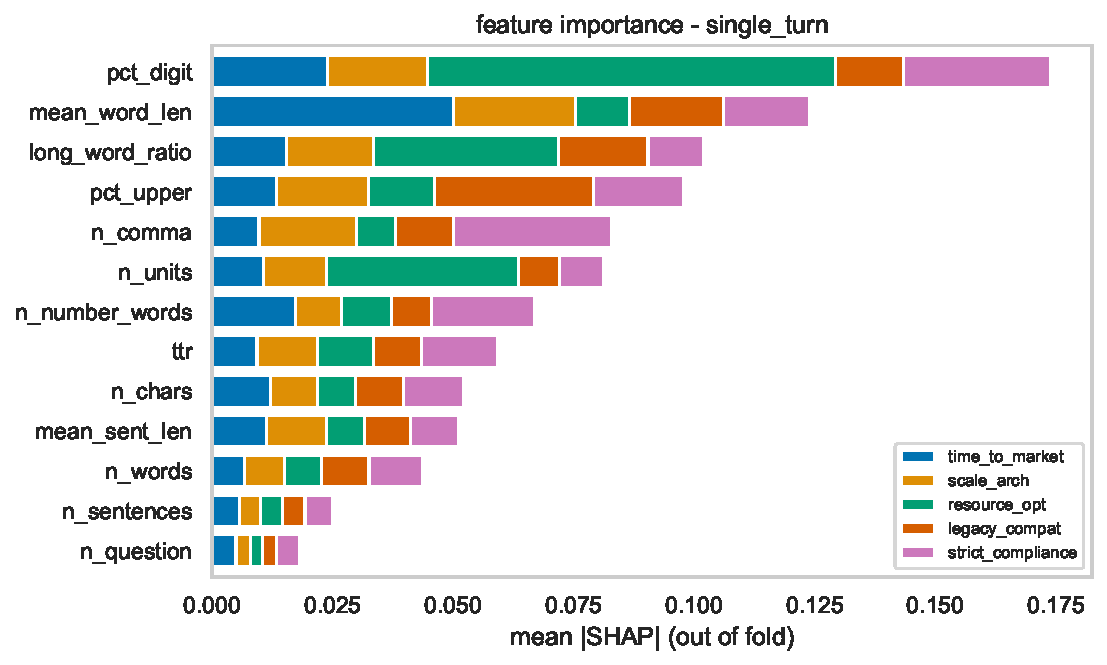
\includegraphics[width=0.9\textwidth]{images/plots/anova/dataset_shap_single_turn.pdf}
    \caption[Mean absolute SHAP value per feature and sub-agent, single-turn dataset]{Mean absolute SHAP value, out of fold, per feature and sub-agent, single-turn dataset.}
    \label{fig:shap-single}
\end{figure}

\begin{figure}[H]
    \centering
    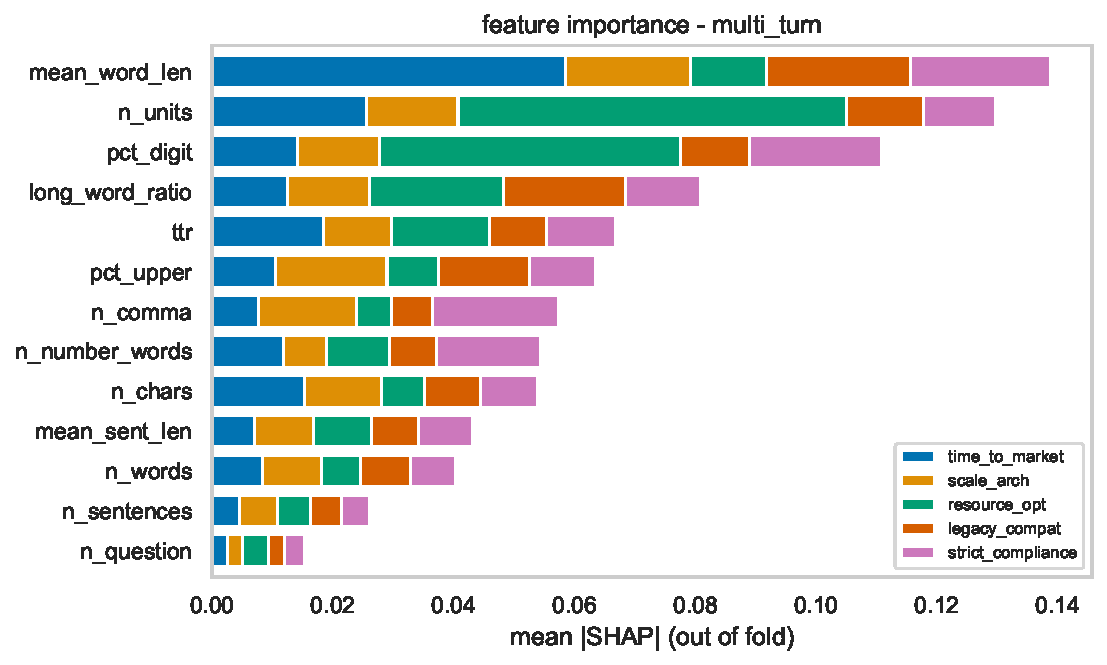
\includegraphics[width=0.9\textwidth]{images/plots/anova/dataset_shap_multi_turn.pdf}
    \caption[Mean absolute SHAP value per feature and sub-agent, multi-turn dataset]{Mean absolute SHAP value, out of fold, per feature and sub-agent, multi-turn dataset.}
    \label{fig:shap-multi}
\end{figure}

\flushbottom

Nearly half of the total SHAP attribution of \texttt{pct\_digit} concentrates on \texttt{resource\_opt} in single-turn (0.0847 of 0.174, 49\%), and the same holds for \texttt{n\_units} (49\% in both single-turn and multi-turn). This concentration is weaker for \texttt{pct\_digit} in multi-turn, at 45\%. No other feature concentrates this strongly on a single sub-agent. This confirms the Games-Howell test result of Section~\ref{subsec:anova-posthoc}. The remaining concentrations are weaker but consistent with the same test: \texttt{mean\_word\_len} concentrates on \texttt{time\_to\_market} (about 40\% in both datasets), and \texttt{n\_comma} concentrates on \texttt{strict\_compliance}.

\subsection{Summary}
\label{subsec:anova-summary}

The one-way ANOVA finds a medium effect of \texttt{gold} on only two of the thirteen surface features, \texttt{pct\_digit} and \texttt{n\_units}, both tied to numeric magnitudes in the request text. Every other feature reaches at most a small effect. The Games-Howell test and the SHAP attribution trace the effect on \texttt{pct\_digit} and \texttt{n\_units} to a single sub-agent: \texttt{resource\_opt} states memory ceilings, cost budgets, and latency figures more often than the other four sub-agents, and \texttt{pct\_digit} and \texttt{n\_units} do not separate those other four sub-agents from each other. The multiway ANOVA finds the \texttt{gold} effect on \texttt{pct\_digit} and \texttt{n\_units} independent of \texttt{difficulty}, \texttt{persona}, \texttt{decoy}, and \texttt{pattern}: almost all interaction tests fail to reject the null hypothesis.

Section~\ref{subsec:lexical-separability} requires the sub-agents to be balanced in writing style, not only in vocabulary, and the analysis in this section shows this requirement is not met exactly: \texttt{pct\_digit}, \texttt{n\_units}, \texttt{mean\_word\_len}, and \texttt{long\_word\_ratio} all differ significantly across \texttt{gold}. The purpose of that requirement is to keep a text-only classifier from routing a request by a stylistic marker instead of by its content. A classifier trained on the thirteen surface features reaches its ceiling accuracy almost entirely from the numeric features alone, 0.313 in single-turn and 0.293 in multi-turn against 0.368 and 0.337 for the full feature set (Section~\ref{subsec:shortcut-classifiers}). Both figures stay well below the bag-of-words baseline of 0.684 and 0.645 (Table~\ref{tab:text-baselines}).

Since the thirteen surface features cannot reach that baseline, the accuracy of the bag-of-words classifier must come from the lexical content of the request, the word choices the surface features do not capture, rather than from its style. Besides the numeric features, only \texttt{mean\_word\_len} and \texttt{long\_word\_ratio} differ significantly across \texttt{gold}, and they add only about 0.05 of accuracy over the numeric features alone (Section~\ref{subsec:shortcut-classifiers}). This residual style imbalance is too small for a text-only classifier to route requests by style at a level that would compromise the purpose of the balance requirement in Section~\ref{subsec:lexical-separability}: keeping a request from being routed by how it is written instead of what it asks.


